% Great thanks for Cezary Sałbut (this latex file is mainly based on his work)

\documentclass[a4paper,12pt,fleqn]{article}


\usepackage[utf8]{inputenc} 
\usepackage{polski}
\usepackage[polish]{babel}
\usepackage[pdftex]{color,graphicx}
\usepackage{subfig}
\usepackage{indentfirst}
\usepackage{booktabs}
\usepackage{tabularx}
\usepackage{multirow}
\usepackage{pdflscape}
\usepackage{array}
\usepackage{amsmath}
\usepackage{appendix}
\usepackage{hyperref}
\hypersetup{
    colorlinks,%
    citecolor=black,%
    filecolor=black,%
    linkcolor=black,%
    urlcolor=blue
}

\usepackage{listings}
\lstset{
	numbers=left, 
	stepnumber=1, 
	basicstyle={\footnotesize \ttfamily},
	language=C, 
	captionpos=b,
	xleftmargin=6mm,
	aboveskip=\medskipamount,
	belowskip=\bigskipamount,
	tabsize=4
}

\usepackage{title-page}

\usepackage[top=28mm, bottom=30mm, left=21mm, right=21mm]{geometry}

\linespread{1.5}		%interlinia

\usepackage{boxedminipage} 
%% change the below lengths to suit your needs: 
\setlength{\fboxrule}{1pt} 
\setlength{\fboxsep}{5pt}



\renewcommand{\appendixtocname}{Dodatki}
\renewcommand{\appendixpagename}{Dodatki}


\widowpenalty=10000
\clubpenalty=10000


\newcommand{\autor}{Jan Kurdel}
\newcommand{\tytulpl}{Identyfikacja nieliniowych obiektów dynamicznych metodą uogólnionej regresji postępującej z ortogonalizacją}
\newcommand{\tytulen}{Identification of nonlinear dynamical objects based on Generalized Orthogonal Forward Regression}
\newcommand{\uczelnia}{POLITECHNIKA WARSZAWSKA}
\newcommand{\wydzial}{Wydział Elektroniki i Technik Informacyjnych}
\newcommand{\instytut}{Instytut Systemów Elektronicznych}
\newcommand{\promotor}{dr inż. Stanisława Jankowskiego}
\newcommand{\praca}{Praca inżynierska}
\newcommand{\miejscerok}{Warszawa, 2012}
\newcommand{\indeks}{214460}

\title{\tytulpl}
\author{\autor}

\begin{document}

\renewcommand{\tablename}{Tabela}

\pagestyle{empty}
\stronatytulowa

\newpage
\setcounter{page}{1}

\newpage
\textbf{\tytulpl} \vspace*{0.2cm} \\
Praca opisuje identyfikację obiektów dynamicznych metodą uogólnionej regresji postępującej z ortogonalizacją. Identyfikacja została przeprowadzona na przykładzie nieliniowego obiektu dynamicznego opisanego równaniem Van der Pola. Jakość modelu została następnie oceniona na podstawie błędu średniokwadratowego predykcji na 100 kroków w przód. Model był testowany dla różnych warunków początkowych. Zastosowana metoda pozwoliła poprawnie odwzorować obiekt dynamiczny.

\vspace*{2cm}
\textbf{\tytulen} \vspace*{0.2cm} \\
The aim of this thesis is to identify nonlinear dynamical objects by the Generalized Orthogonal Forward Regression method. The identification was based on a nonlinear dynamical object described by the Van der Pol differential equation.  The quality of a model was evaluated on the basis of mean squared error of 100-step ahead prediction. The model was tested for the set of different initial conditions. The use of the chosen method resulted in obtaining the proper model of the dynamical object.

\newpage
\tableofcontents

\newpage
\pagestyle{plain}

\section{Cel pracy}
	Model matematyczny obiektu opisuje związek między sygnałem podawanym na wejście (sterowaniem) oraz sygnałem wyjściowym. Modelowanie takie wykorzystuje się pracując nad silnikami, robotami przemysłowymi, klimatyzacją, systemami hamulcowymi\cite{Isermann}. Oprócz szerokiego spektrum dziedzin, w których ma zastosowanie tworzenie modeli, istnieje szereg różnych metod ich tworzenia na postawie danych doświadczalnych, czyli metod identyfikacji obiektów.
	
	Podstawą metod identyfikacji jest wykorzystanie charakterystyk czasowych bądź charakterystyk częstotliwościowych w celu znalezienia zależności między wejściem a wyjściem obiektu\cite{Czemplik}.
	
	W pracy zdecydowano się na inną metodę identyfikacji dynamiki obiektu - wykorzystano w tym celu sieć neuronową. Można spotkać się z wieloma przykładami zastosowania sieci neuronowych w zadaniu identyfikacji obiektu dynamicznego, jednak struktura oraz algorytmy trenowania takiej sieci  mogą znacznie się różnić. W pracy zostanie przedstawiona metoda uogólnionej regresji postępującej z ortogonalizacją (Generalized Orthogonal Forward Regression - GOFR) oraz jej wykorzystanie do identyfikacji nieliniowego obiektu dynamicznego opisanego równaniem różniczkowym Van der Pola. Następnie zostanie dokonana ocena jakości modelowania z wykorzystaniem zaproponowanego rozwiązania. W tym celu zostanie opracowany program implementujący przedstawioną metodę wraz z przykładem jej wykorzystania. Równanie Van der Pola ma zastosowanie między innymi w dziedzinie układów elektronicznych\cite{Palczewski}. Należy zaznaczyć, że zaproponowany algorytm może mieć zastosowanie również do obiektów opisanych innymi równaniami różniczkowymi.  

\newpage
\section{Dynamika obiektów}
Układ dynamiczny to matematyczny model, który opisuje ewolucję realnego zjawiska. Model taki pozwala na analizę reakcji badanego obiektu na pojawiające się zmiany.
Układ dynamiczny z czasem ciągłym jest opisywany układem równań ruchu w postaci ogólnej\cite{Kosinski}
\begin{equation}
	\frac{dx}{dt} = F(x,r), \quad x \in R
\end{equation}

gdzie: \\
$F$ - odwzorowanie $F:U \rightarrow R^n$,
$r$ - zbiór parametrów kontrolnych układu,
$U$ – podzbiór $R^n$ określający przestrzeń fazową układu.

Przestrzeń fazowa jest przestrzenią wszystkich możliwych stanów w jakich może znajdować się badany układ. Każdy stan układu jest pojedynczym punktem tej przestrzeni. Konkretne rozwiązanie układu równań ruchu $\phi_i(t_0,r)$ - dla danych wartości parametrów $r$ i warunków początkowych zwane jest orbitą (trajektorią). Jeśli odwzorowanie $F$ jest odwzorowaniem liniowym to układ dynamiczny jest układem liniowym, natomiast jeśli $F$ jest odwzorowaniem nieliniowym to układ dynamiczny nazywamy układem nieliniowym.

Uniwersalnym sposobem opisu dynamiki obiektów z czasem ciągłym są równania różniczkowe. Dla opisu dynamiki obiektów z czasem dyskretnym odpowiednio stosowane są równania różnicowe\cite{Gutenbaum}.
\subsection{Równania różniczkowe zwyczajne}

Równaniem różniczkowym zwyczajnym nazywamy równanie zawierające zmienną niezależną $x$, nieznaną funkcję $y$, oraz jej pochodne $y', y'', \hdots, y^{(n)}$ \cite{BCh_2001}
\begin{equation}
	\label{wzor:rownanie_roz_N_stopnia}
	F(x,y,y',\hdots,y^{(n)}) = 0
\end{equation}
gdzie $F:R^{n+2} \rightarrow R$

Warunek początkowy (Cauchy'ego) dla równania \eqref{wzor:rownanie_roz_N_stopnia} określony jest poprzez: 
\begin{equation}
\begin{array}{c}
y(x_0)       =  y_0,     \\
y'(x_0)      =  y_1,     \\
\vdots			   	     \\
y^{n-1}(x_0) = y_{n-1}
\end{array}
\end{equation}
gdzie $y_0, y_1, \hdots, y_{n-1}$ są zadanymi liczbami.

Stopień pochodnej w równaniu \eqref{wzor:rownanie_roz_N_stopnia} określa rząd równania różniczkowego. Równanie różniczkowe pierwszego rzędu wyraża się zatem wzorem:
\begin{equation}
	\label{wzor:rownanie_roz_I_stopnia}
	y' = f(x,y)
\end{equation}

Równanie \eqref{wzor:rownanie_roz_I_stopnia} może zostać rozwiązane numerycznie na wiele sposobów. Można wyróżnić podział na metody jednokrokowe, które wymagają jedynie informacji z poprzedniego kroku (zatem warunek początkowy jest wystarczający do obliczenia równania różniczkowego dla kolejnego punktu) oraz metody wielokrokowe, w których rozwiązanie jest dokonowywane z wykorzystaniem znajomości kilku poprzednich kroków. Wśród metod jednokrokowych znajdują się m.in. metody Eulera oraz Rungego-Kutty.

\subsection{Metody rozwiązywania równań różniczkowych}

\subsection*{Metoda Eulera}
Metoda Eulera jest najprostszą metodą numeryczną rozwiązywania równań różniczkowych. Mając dane równanie \eqref{wzor:rownanie_roz_I_stopnia} oraz warunek początkowy postaci:
\begin{equation}
	y(x_0) = y_0	
\end{equation}
poszukujemy rozwiązania dla kolejnego momentu $x_1 = x_0 + h$, gdzie $h$ jest krokiem metody. W~tym celu możemy skorzystać z rozwinięcia w szereg Taylora w pobliżu punktu początkowego $x_0$:
\begin{equation}
	y(x_0 + h) = y(x_0) + hy'(x_0) + \frac{h^2}{2!}y''(x_0) + \hdots
\end{equation}
Korzystając tylko z dwóch pierwszych elementów szeregu Taylora otrzymamy:
\begin{equation}
	y(x_0 + h) = y(x_0) + hy'(x_0) = y(x_0) + hf(x_0,y_0)
\end{equation}
Powtarzając tę czynność wielokrotnie otrzymamy wzór:
\begin{equation}
	y_{n+1} = y_{n} + hf(x_n,y_n)
\end{equation}
określany jawną metodą Eulera.

\subsection*{Metoda Rungego-Kutty}
Kolejną metodą numerycznego rozwiązywania równań różniczkowych jest metoda Rungego-Kutty, która jest metodą wieloetapową. W każdym kroku konieczne jest obliczenie wartości funkcji $f$ dla różnych argumentów. Wśród metod Rungego-Kutty można wyróżnić różne warianty tej metody w zależności od rzędu metody. Najprostszą z nich jest metoda Rungego-Kutty rzędu II. Przyjmuje ona postać:
\begin{equation}
	y_{i+1} = y_i + \frac{h}{2}(k_1 + k_2)
\end{equation}
gdzie \\ \hspace*{0.8cm}
$\begin{array}{l}
	k_1 = f(t_i,y_i) \\
	k_2 = f(t_i + h, y_i + hk_1)
\end{array}$ \\

Najbardziej popularną jest metoda rzędu IV, która przyjmuje postać:
\begin{equation}
	y_{i+1} = y_i + \frac{h}{6}(k_1 + 2k_2 + 2k_3 + k_4)
\end{equation}
gdzie \\ \hspace*{0.8cm}
$\begin{array}{c}
	k_1 = f(t_i,y_i) \\
	k_2 = f(t_i + \frac{h}{2}, y_i + \frac{h}{2}k_1) \\
	k_3 = f(t_i + \frac{h}{2}, y_i + \frac{h}{2}k_2) \\
	k_4 = f(t_i + h,y_i + hk_3) \\
\end{array}$ \\

\subsection*{Równania różniczkowe zwyczajne wyższych rzędów}
Równanie różniczkowe wyższych rzędów może zostać sprowadzone do układu równań różniczkowych rzędu pierwszego \cite{AK_RBG2002}. Mając dane równanie różniczkowego n-tego rzędu: \\ \hspace*{0.8cm} 
$y^{(n)}(t) = f(t,y(t),y'(t),\hdots,y^{(n-1)}(t)), \qquad a \leq t \leq b$ \\
z warunkiem początkowym w postaci: \\ \hspace*{0.8cm}

$\begin{array}{l}
y(a)       = \alpha_0,    \\
y'(a)      = \alpha_1,    \\
\vdots					  \\
y^{n-1}(a) = \alpha_{n-1} \\
\end{array}$ \\

oraz wprowadzając nowe zmienne: \\ \hspace*{0.8cm}
$y_1(t) = y(t), y_2(t) = y'(t), \hdots, y_n(t) = y^{(n-1)}(t)$

otrzymujemy układ równań różniczkowych pierwszego rzędu postaci: \\ \hspace*{0.8cm}
$\begin{array}{l}
y'_1       = y_2   \\
y'_2       = y_3   \\
\vdots			   \\
y'_{n-1} = y_n     \\
y'_n = f(t,y_1,y_2,\hdots,y_n)
\end{array}$ \\

z warunkami początkowymi postaci: \\ \hspace*{0.8cm}
$y_1(a) = \alpha_0, y_2(a) = \alpha_1, \hdots, y_n(a) = \alpha_{n-1}$ 

Dzięki takiemu zabiegowi możliwe jest rozwiązanie równania różniczkowego wyższego rzędu metodami służącymi do rozwiązywania równań różniczkowych rzędu pierwszego.

Należy zaznaczyć, że wymienione metody rozwiązywania równań różniczkowych mogą mieć zastosowanie jedynie w przypadku znajomości postaci równania różniczkowego.
 
\newpage
\section{Sieci neuronowe} 

Sztuczne sieci neuronowe mają bardzo szerokie zastosowanie. Wykorzystywane są m. in do zadań klasyfikacji, aproksymacji, predykcji, sterowania w wielu różnych dziedzinach życia. Definicja sieci neuronowej nie została dokładnie sprecyzowana, ale sieci neuronowe można określić jako adaptacyjne metody tworzenia modeli nieliniowych na podstawie danych eksperymentalnych, bądź też formalne modele statystyczne zbudowane na podstawie danych eksperymentalnych~\cite{Jankowski}.
 
\subsection{Struktura sieci neuronowych}
Podstawą jednostką sieci neuronowych jest neuron. Budowa neuronu jest przedstawiona na rysunku \ref{fig:neuron}. Neuron taki sumuje sygnał podany na jego wejścia $x_i$ z odpowiednimi wagami $w_i$, dając na wyjście wynik $y$ sumy przeprowadzonej przez funkcję aktywacji $f(x)$.
\begin{figure}[ht!]
	\centering
	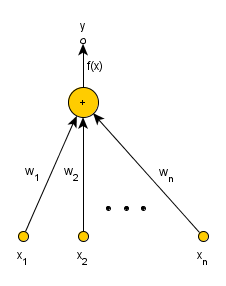
\includegraphics[scale=0.8]{images/single_neuron.png}
	\caption{Postać neuronu}
	\label{fig:neuron}
\end{figure}

Sieć neuronową tworzą grupy połączonych ze sobą neuronów. Podstawową sieć neuronową stanowi perceptron wielowarstwowy przedstawiony na rysunku  \ref{fig:multilayer}. Pierwsza warstwa nosi nazwę warstwy wejściowej (\textit{Input}), ostatnia warstwa sieci nosi nazwę warstwy wyjściowej (\textit{Output}). Wszystkie pozostałe warstwy noszą nazwę warstw ukrytych (\textit{Hidden}).

\begin{figure}
	\centering
	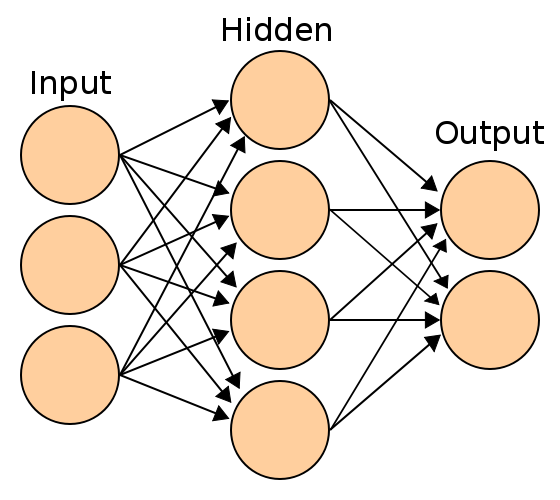
\includegraphics[width=0.5\textwidth]{images/560px-Artificial_neural_network.png}
	\caption{Schemat budowy perceptronu wielowarstwowego \\
	\footnotesize{\textit{źródło:} \url{http://commons.wikimedia.org/wiki/File:Artificial\_neural\_network.svg}} }
	\label{fig:multilayer}
\end{figure}

Funkcja aktywacji często przyjmuje postać $f(x) = \frac{1}{1 + \exp(-\beta x)}$ określanej mianem funkcji unipolarnej, bądź też $f(x) = tgh(\beta x)$ określanej mianej funkcji bipolarnej.
 
\subsubsection*{Sieć RBF}
Sieć RBF (Radial Basis Function) jest sztuczną siecią neuronową o radialnych funkcjach bazowych. Sieć ta ma szerokie zastosowanie i jest wykorzystywana m.in. do modelowania 3D, rozpoznawania mowy, identyfikacji systemów, modelowania parametrów urządzeń elektronicznych\cite{Bors}. Sieć taka składa się zazwyczaj z jednej warstwy ukrytej, gdzie funkcja aktywacji jest radialną funkcją bazową oraz warstwy wyjściowej w postaci neuronu liniowego. Radialna funkcja bazowa jest określona w sposób następujący~\cite{Bartkowiak}
\begin{equation}
	G(x,c) = G(r(x,c))
\end{equation}
gdzie $r(x,c)$ jest odległością między punktami $r$ i $c$, a centrum $c$ jest ustalone i pełni rolę parametru funkcji. Jedną z bardziej popularnych radialnych funkcji bazowych jest funkcja Gaussa:
\begin{equation}
	G(r) = \exp(\frac{-r^2}{2\sigma^2})
\end{equation}
Często w sieciach RBF stosowane są również następujące funkcje bazowe\cite{Chen}: \\
$\begin{array}{l}
 G(r) = r^2 log(r)\\
 G(r) = (r^2 + \sigma^2)^{\frac{1}{2}} \\
 G(r) = (r^2 + \sigma^2)^{-\frac{1}{2}}
\end{array}
$
\subsection{Metody gradientowe uczenia sieci}
Do najbardziej skutecznych metod uczenia sieci neuronowych należą metody gradientowe. Algorytmy te bazują na rozwinięciu w szereg Taylora funkcji celu $E(W)$ w najbliższym sąsiedztwie znanego rozwiązania\cite{Osowski}.
\begin{equation}
	\label{wzor:metoda_gradientowa}
	E(w + p) = E(w) + [(g(w)]^Tp + \frac{1}{2}p^TH(w)p + \hdots
\end{equation}
gdzie
$$g(w) = \nabla E = [\frac{\partial E}{\partial w_1}, \frac{\partial E}{\partial w_2}, \hdots, \frac{\partial E}{\partial w_n}]^T$$
$$H(w) = \begin{bmatrix}
\frac{\partial^2 E}{\partial w_1 \partial w_2} & \hdots & \frac{\partial^2 E}{\partial w_1 \partial w_n}\\
\vdots & & \vdots \\
\frac{\partial^2 E}{\partial w_n \partial w_1} & \hdots & \frac{\partial^2 E}{\partial w_n \partial w_n}
\end{bmatrix}$$
$\nabla E$ jest wektorem pierwszych pochodnych - gradientem, natomiast $H(w)$ jest macierzą drugich pochodnych - hesjanem. W praktyce są używane co najwyżej 3 pierwsze elementy równania~\eqref{wzor:metoda_gradientowa}. W metodzie gradientowej poszukuje się minimum funkcji celu poprzez taką aktualizację wektora kierunkowego $p$ oraz kroku $\eta$ dla punktu $w_{k+1} = w_k + \eta_k p_k$ aby prawdziwa była nierówność $E(w_{k+1}) < E(w_k)$.

\subsubsection*{Algorytm największego spadku}
Metoda największego spadku chociaż jest metodą wolno zbieżną to warto ją omówić ze względu na jej prostotę. Ograniczając się do liniowej aproksymacji funkcji celu opisanej równaniem \eqref{wzor:metoda_gradientowa} zapisanej w postaci rozwinięcia szeregu Taylora otrzymujemy wzór:
\begin{equation}
	E(w_{k+1}) = E(w) + [(g(w)]^Tp
\end{equation} 
Aby była spełniona nierówność $E(w_{k+1}) < E(w_k)$ wystarczy spełnić warunek $[(g(w)]^Tp < 0$. Wektor kierunkowy spełniający nierówność wynosi $p = -[g(w)]^T$. Graficznie działanie algorytmu przedstawia rysunek \ref{fig:gradient}. Czerwoną linią została przedstawiona funkcja kosztu $E(w)$ jako funkcja jednej zmiennej $w$. Zieloną linią została oznaczona styczna do wykresu w punkcie $w_k$, gdzie pochodna jest mniejsza od zera. W tym przypadku należy przemieścić się w stronę dodatnich wartości $w$ czyli zgodnie z kierunkiem $-\frac{dE}{dw}$. Niebieską linią została oznaczona styczna do wykresu w punkcie $w_k$, gdzie pochodna jest większa od zera. W tym przypadku należy przemieścić się w stronę ujemnych wartości $w$ czyli również zgodnie z kierunkiem $-\frac{dE}{dw}$.

\begin{figure}
	\centering
	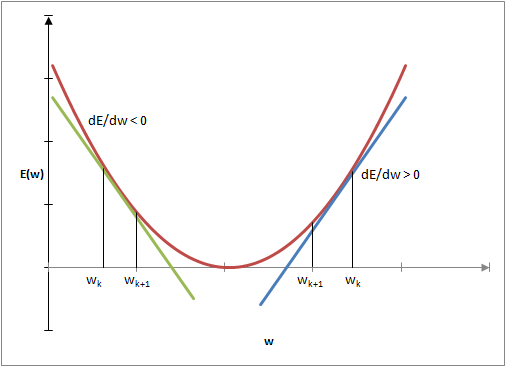
\includegraphics[width=0.8\textwidth]{images/gradient.png}
	\caption{Funkcja kosztu}
	\label{fig:gradient}
\end{figure}

\subsubsection*{Algorytm Levenberga-Marquardta}
Podczas gdy wcześniej nie została określona konkretna funkcji celu, tak w przypadku algorytmu Levenberga-Marquardta funkcją celu jest błąd średniokwadratowy (MSE)\cite{Bishop}
\begin{equation}
	\label{wzor:mse}
	E = \frac{1}{2} \sum_{n=1}^N(e_n)^2 = \frac{1}{2} \sum_{n=1}^N(y_n - \tilde{y_n})^2
\end{equation}
gdzie $e_n$ jest błędem n-tego wzorca, $y_n$ n-tym wzorcem, $\tilde{y_n}$ wyjściem sieci dla n-tego wzorca.

Zakładając, że aktualnie jesteśmy w punkcie $w_{i}$ i chcemy przemieścić się do punktu $w_{i+1}$, który jest niedaleko oddalony od $w_{i}$, w celu obliczenia nowej wartości błędu $e$ możemy skorzystać z rozwinięcia w szereg Taylora:
\begin{equation}
	\label{wzor:blad_lm}
	e(w_{i+1}) = e(w_{i}) + Z(w_{i+1} - w_{i})
\end{equation}
gdzie $Z \equiv \nabla e$. Po podstawieniu równania \eqref{wzor:blad_lm} do równania \eqref{wzor:mse} wzór na błąd średniokwadratowy może zostać zapisany jako:
\begin{equation}
	\label{wzor:mse2}
	E = \frac{1}{2}[e(w_{i}) + Z(w_{i+1} - w_{i})]^2
\end{equation}
Chcą zminimalizować równanie \eqref{wzor:mse2} ze względu na zmienną $w_{i+1}$ otrzymujemy wzór:
\begin{equation}
	w_{i+1} = w_{i} - (Z^TZ)^{-1}Z^Te(w_{i})
\end{equation}
Jednak taki sposób obliczania $w_{i+1}$ może powodować, że krok $w_{i+1} - w_{i}$ będzie duży a wtedy liniowa aproksymacja szeregiem Taylora może stać się niedokładna. Z tego powodu algorytm Levenberga-Marquardta korzysta ze zmodyfikowanej funkcji celu w postaci:
\begin{equation}
	\label{wzor:mse_lm}
	E = \frac{1}{2}(e(w_{i}) + Z(w_{i+1} - w_{i}))^2 + \lambda (w_{i+1} - w_{i})^2
\end{equation}
Chcą zminimalizować równanie \eqref{wzor:mse_lm} otrzymujemy ostatecznie równanie opisujące sposób obliczania wag w kolejnych iteracjach dla algorytmu Levenberga-Marquardta:
\begin{equation}
	w_{i+1} = w_{i} -(Z^TZ + \lambda I)^{-1}Z^Te(w_{i})
\end{equation}
gdzie $I$ jest macierzą jednostkową. Wartość $\lambda$ zmienia się w trakcie obliczania kolejnych wartości $w_{i+1}$. Jeśli błąd $E$ zmniejsza się wartość $\lambda$ jest zmniejszana o określony współczynnik. W~przypadku wzrostu wartości błędu wartość $\lambda$ jest zwiększana o określony współczynnik oraz ponownie przyjmowana jest wartość $w_i$.



\newpage
\section{Selekcja funkcji bazowych z wykorzystaniem metody GOFR}
W przypadku sieci RBF problem może stanowić wybór odpowiednich funkcji bazowych oraz odpowiedniej ich ilości. Zbyt mała ilość funkcji nie pozwoli na wystarczające zminimalizowanie błędu sieci na zbiorze uczącym. Z kolei zbyt duża ilość funkcji może doprowadzić do problemu nadmiernego dopasowania a co za tym idzie sieć traci zdolność do generalizacji. Jedną z metod rozwiązania tego problemu jest zastosowanie metody GOFR opartej o metodę OLS (Orthogonal Least Square). 

\subsection{Selekcja z wykorzystaniem ortogonalizacji oraz metody najmniejszych kwadratów}
Jedną z metod selekcji najbardziej znaczących funkcji bazowych jest metoda oparta o metodę najmniejszych kwadratów oraz ortogonalizację (OLS)\cite{Chen}. Metoda ta umożliwia określenie wkładu każdej funkcji bazowej i wybranie tych najbardziej istotnych. Mając dany wektor wag sieci $w = [w_0, w_1, \hdots, w_K]^T$ oraz wektor danych uczących $d = [d_1, d_2, \hdots, d_p]^T$ można zapisać macierz G w postaci:
\begin{equation}
G = \begin{bmatrix}
\phi_{11} & \phi_{21} & \hdots & \phi_{K1} \\
\phi_{12} & \phi_{22} & \hdots & \phi_{K2} \\
\hdots    & \hdots    & \hdots & \hdots    \\
\phi_{1p} & \phi_{2p} & \hdots & \phi_{Kp}
\end{bmatrix}
\end{equation}
gdzie $\phi_{ji}$ oznacza odpowiedź i-tej funkcji radialnej na j-ty wzorzec uczący. Oznaczając przez $g_i = [g_{i1}, g_{i2}, \hdots, g_{ip}]^T$ odpowiedź i-tej funkcji radialnej na wszystkie wzorce uczące można macierz G przedstawić w postaci:
\begin{equation}G = [g_1, g_2, \hdots, g_K] \end{equation}
Dla takich oznaczeń, dla sieci RBF można zapisać następujące równanie:
\begin{equation}
\label{wzor:ofr_rbf}
d = Gw + e\end
{equation}
gdzie $e$ jest błędem aproksymacji. Ortogonalizacja macierzy G pozwala na określenie osobno wpływu każdej funkcji $g_i$ na wartość części pożądanej energii zdefiniowanej jako $(Gw)^2$ \cite{Osowski}. Dzięki temu możliwa jest selekcja najbardziej istotnych funkcji bazowych oraz znaczne ograniczenie ilości funkcji tworzących sieć. Sama ortogonalizacja może zostać dokonana różnymi metodami np. metodą Grama-Schmidta, gdzie w procesie ortogonalizacji macierzy $G$ powstaje macierz ortogonalna $Q$ oraz macierz górnotrójkątna $A$.
\begin{equation}G = QA\end{equation}
\begin{equation}
A = \begin{bmatrix}
1      & a{12}  & a{13}  & \hdots & a_{1K} \\
0      & 1      & a{23}  & \hdots & a_{2K} \\
\hdots & \hdots & \hdots & \hdots & \hdots \\
0      & 0      & 0      & 0      & 1     
\end{bmatrix}
\end{equation}
Po procesie ortogonalizacji oraz wprowadzając nowe oznaczenie $b = Aw$ można zapisać nową postać równania \eqref{wzor:ofr_rbf}:
\begin{equation}
	\label{wzor:ofr_rbf2}
	d = QAw + e = Qb + e
\end{equation}
Rozwiązując równanie \eqref{wzor:ofr_rbf2} metodą najmniejszych kwadratów otrzymujemy:
\begin{equation}
	b = (QQ^T)^{-1}Q^Td
\end{equation}
Mając dane $b$ oraz $A$ jesteśmy w stanie określić wektor wag $w = A^{-1}b$.
Jak wspomniano wcześniej wartość pożądana energii jest określona jako $(Gw)^2$. Na tej podstawie można zdefiniować wzór określający udział danej funkcji w ogólnym bilansie energii jako:
\begin{equation}
	\epsilon_i = \frac{b_i^2q_i^Tq_i}{d^Td}
\end{equation}

Warunek stopu metody może zostać określony m. in. poprzez doprowadzenie do sytuacji, gdzie wartość sumaryczna energii wnoszonej przez wszystkie funkcje będzie bliska jedności, czyli:
\begin{equation}
	1 - \sum_{i=1}^N \epsilon_i < \delta
\end{equation}
gdzie $\delta$ jest z góry ustaloną wielkością warunkując koniec algorytmu.

Jak wspomniano wcześniej ortogonalizacja może zostać wykonana różnymi metodami, jednak omówiona zostanie metoda ortogonalizacji Grama-Schmidta ze względu na jej popularność. Stosując algorytm ortogonalizacji Grama-Schmidta można dokonać rozkładu QR macierzy A, gdzie macierz Q jest macierzą ortogonalną zaś macierz R jest macierzą górnotrójkątną z jedynkami na diagonali. Algorytm takiego rozkładu można przedstawić w sposób następujący\cite{Bernardelli}:
\begin{equation}
	\begin{array}{l}
	q_1 = a_1 \\
	q_k = a_k - \sum_{j=1}^{k-1} r_{jk}q_j = a_k - \sum_{j=1}^{k-1} \frac{<a_k,q_j>}{<q_j,q_j>} q_j, \quad 2 \leq l  \leq n 
\end{array}
\end{equation}
$\frac{<a_k,q_j>}{<q_j,q_j>} q_j$ jest rzutowaniem ortogonalnym wektora $a_k$ na wektor $q_j$.

Graficzna reprezentacja procesu ortogonalizacji dla dwóch pierwszych kroków przedstawiona jest na rysunku \ref{fig:gram}. Mając wybrany wektor $u_1$ (literą $e$ oznaczono znormalizowany wektor $u$) należy dokonać projekcji (rzutu ortogonalnego) kolejnego wektora na przestrzeń rozpiętą przez wszystkie ortogonalne wektory (w tym przypadku tylko wektor $u_1$). Różnica wektora ortogonalizowanego oraz projekcji wektora ortogonalizowanego ($proj_{u_1}v_2$)na przestrzeń rozpiętą przez wektory ortogonalne pozwala uzyskać nam kolejny wektor ortogonalny ($u_2$).
\begin{figure}[ht!]
	\centering
	
	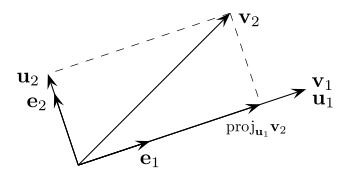
\includegraphics[scale=0.7]{images/GramSchmidt.png}
	\caption{Proces ortogonalizacji dla dwóch pierwszych kroków metody Grama-Schmidta \\
	\footnotesize {\textit{źródło:} \url{http://commons.wikimedia.org/wiki/File:Gram\%E2\%80\%93Schmidt\_process.svg}}}
	\label{fig:gram}	

\end{figure}

Funkcje wybiera się spośród wcześniej wygenerowanej biblioteki funkcji. Metoda ta zapewnia wybór najbardziej optymalnego zbioru funkcji z biblioteki. Jednak aby wybór ten był optymalny konieczne jest wygenerowanie odpowiedniej biblioteki, która może zawierać znaczną ilość funkcji bazowych przez co proces uczenia się sieci może stać się nieefektywny. Rozwiązaniem w tym przypadku jest zastosowanie metody GOFR

\subsection{Selekcja metodą uogólnionej regresji postępującej z ortogonalizacją (GOFR)}
Metoda GOFR oparta jest na metodzie OLS\cite{Duboisa}. Modyfikację w stosunku do metody OLS stanowi optymalizacja dokonywana na etapie selekcji każdej funkcji bazowej. Optymalizacja ta polega na minimalizacji błędu sieci na zbiorze uczącym (np. zdefiniowanego jako MSE), poprzez odpowiedni dobór parametrów każdej wybranej funkcji. Optymalizacja taka może zostać przeprowadzona metodą gradientową.

Porównanie obu metod przedstawia schemat z rysunku \ref{img:ofr_and_gofr}. Linią przerywaną na rysunku \ref{img:gofr} zaznaczony jest krok specyficzny dla metody GOFR. Optymalizacja pozwala na zmniejszenie ilości funkcji tworzących bibliotekę. Dzieje się tak dzięki temu, że po wyborze odpowiedniej funkcji algorytm zmodyfikuje parametry wybranej funkcji tak aby zminimalizować błąd. W przypadku algorytmu opartego o OLS parametry funkcji były stałe, a ilość funkcji tworzących bibliotekę musiała być duża w celu zapewnienia odpowiednio wysokiego prawdopodobieństwa wyboru optymalnych funkcji bazowych.

\begin{figure}[ht!]
	\centering

	\subfloat[OFR]
	{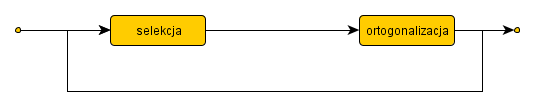
\includegraphics[width=0.8\textwidth]
	{images/ofr.png}
	\label{img:ofr}}
	
	\subfloat[GOFR]
	{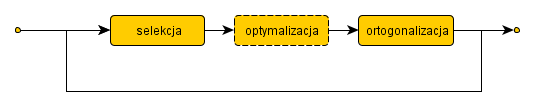
\includegraphics[width=0.8\textwidth]
	{images/gofr.png}
	\label{img:gofr}}
	
	\caption{Porównanie metod OFR oraz GOFR}
	\label{img:ofr_and_gofr}
\end{figure}

\clearpage
\section{Identyfikacja obiektu opisanego równaniem \mbox{Van der Pola}}

Równanie różniczkowe Van der Pola jest określone jako:
\begin{equation}
	\label{wzor:van_der_pol}
	y''(t) - \mu(1 - y^2(t))y'(t) + y(t) = 0
\end{equation}

Jest to podstawowy model procesu oscylacji w fizyce, elektronice, biologii, neurologii, socjologii i ekonomii\cite{Tsatsos}.

Identyfikację obiektu opisanego równaniem \eqref{wzor:van_der_pol} (dla $\mu = 1$) przeprowadzono z użyciem sieci RBF i metody GOFR selekcji funkcji bazowych. Strukturę zaproponowanej sieci przedstawia rysunek~\ref{fig:rbf}.
\begin{figure}[ht!]
	\centering
	
	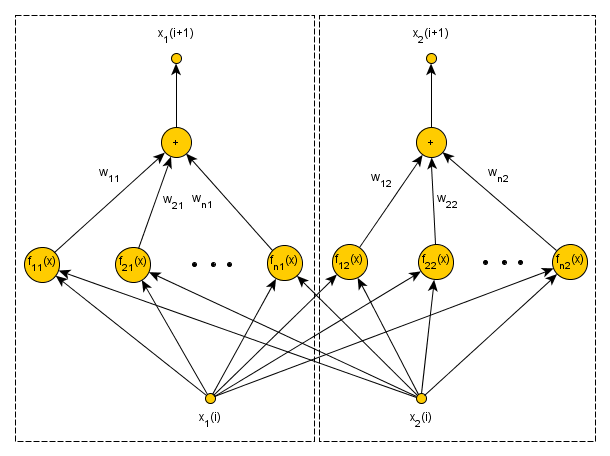
\includegraphics[width = \textwidth]{images/rbf.png}
	\caption{Schemat zaprojektowanej sieci RBF}
	\label{fig:rbf}	

\end{figure}
Wejście sieci stanowią $x_1 = y(t)$ oraz $x_2 = y'(t)$, czyli aktualny stan obiektu. Wyjściem sieci jest stan obiektu w kolejnym kroku. Jak można zauważyć sieć została podzielona na dwie do pewnego stopnia niezależne części - każde z wejść posiada oddzielny zbiór funkcji RBF. W~związku z tym każda z części sieci była uczona oddzielnie (dla tych samych danych uczących). 

Zbiór danych uczących sieć neuronową wygenerowano rozwiązując równanie metodą Rungego-Kutty czwartego rzędu dla warunków początkowych [$y(0)=0,y'(0)=2$], kroku metody $h=0.1$, w~przedziale $t \in [0,50]$. Równanie różniczkowe \eqref{wzor:van_der_pol} drugiego rzędu zapisano w postaci układu dwóch równań różniczkowych pierwszego rzędu:
\begin{equation}
	\begin{array}{l}
    y'(t)  = y_1 \\
    y_1'(t) = (1-y_1^2)y-y_1
    \end{array}
\end{equation}

Powstała w wyniku rozwiązania równania Van der Pola trajektoria, wykres funkcji $y(t)$ oraz jej pierwszej pochodnej $y'(t)$ przedstawione są odpowiednio na rysunkach \ref{img:traj}, \ref{img:func} oraz \ref{img:first_deriv}. Dane powstałe w wyniku rozwiązania równania zostały użyte jako zbiór danych uczących (po odrzuceniu danych z przedziału $t \in [0,10]$ w celu pominięcia stanów nieustalonych).

\begin{figure}[ht!]
	\centering

	\subfloat[Trajektoria]
	{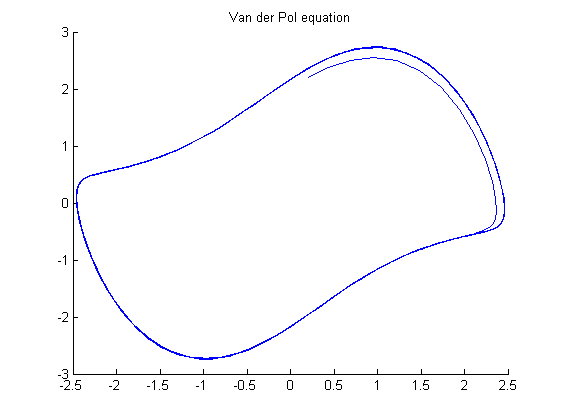
\includegraphics[width=0.5\textwidth]
	{images/trajectory.png}
	\label{img:traj}}
	\subfloat[Wykres funkcji $y(t)$]
	{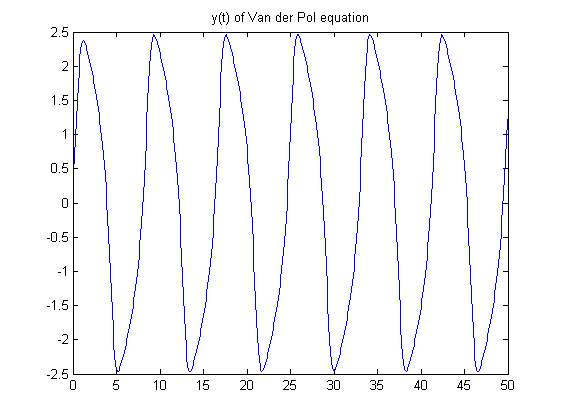
\includegraphics[width=0.5\textwidth]
	{images/signal.png}
	\label{img:func}}
	
	\subfloat[Wykres pierwszej pochodnej $y'(t)$]
	{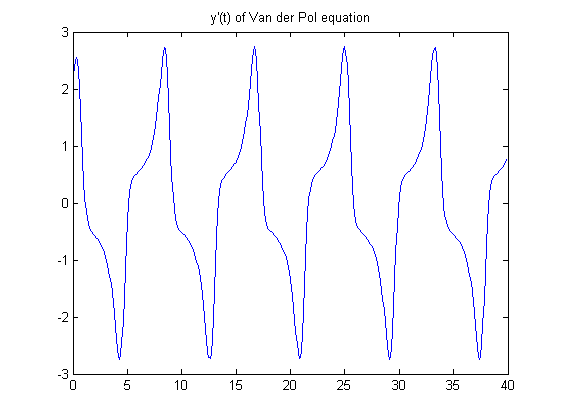
\includegraphics[width=0.45\textwidth]
	{images/first_deriv.png}
	\label{img:first_deriv}}
	
	\caption{Rozwiązanie równania różniczkowego Van der Pola dla warunków początkowych [$y(0)=0,y'(0)=2$]}
\end{figure}

Kolejnym etapem było stworzenie odpowiedniej biblioteki funkcji RBF. W tym celu najpierw wygenerowano bibliotekę 115 funkcji RBF postaci:
\begin{equation}
	\label{wzor:rbf_2d}
	f(x_1(t),x_2(t),c_1,c_2,\sigma) = \exp(-\frac{(x_1(t)-c_1)^2 + (x_2(t)-c_2)^2}{2 \sigma^2})\
\end{equation} gdzie: \\
$x_1(t) = y(t)$ \\
$x_2(t) = y'(t)$ \\

Generowanie biblioteki odbywało się poprzez wybór równomiernie rozłożonych w przestrzeni dwuwymiarowej $D = [min(x_1),max(x_1)] \times [min(x_2),max(x_2)]$ centrów. Dla każdego kolejnego poziomu generowania biblioteki funkcji, nowe centra $c_1$ oraz $c_2$ były wybierane poprzez dwukrotnie zagęszczenie punktów w każdej z osi oraz zmniejszanie szerokości funkcji gaussa $\sigma$ o połowę. Centra dla tak wygenerowanych funkcji przedstawia rysunek \ref{img:rbf_centers}. Ilość poziomów ograniczono do trzech, generując w ten sposób 115 funkcji RBF.

\begin{figure}[ht!]
	\centering	
	
	\subfloat[poziom 1]
	{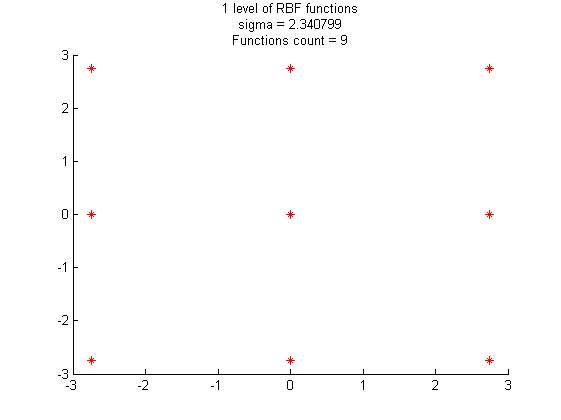
\includegraphics[width=0.33\textwidth]
	{images/centers1.png}}
	\subfloat[poziom 2]
	{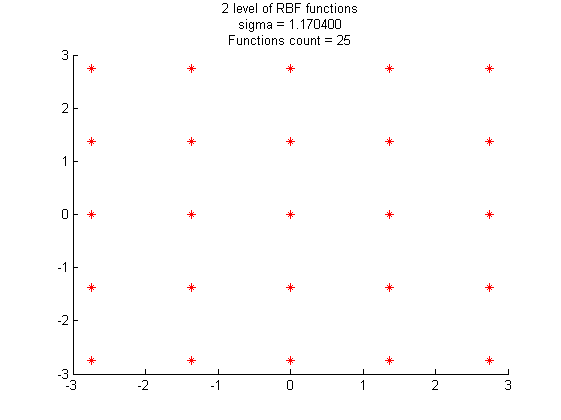
\includegraphics[width=0.33\textwidth]
	{images/centers2.png}}
	\subfloat[poziom 3]
	{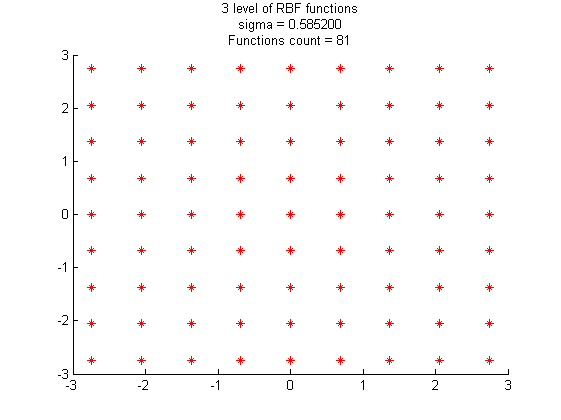
\includegraphics[width=0.33\textwidth]
	{images/centers3.png}}

	\caption{Centra wygenerowanych funkcji RBF dla 3 poziomów}
	\label{img:rbf_centers}
\end{figure}

Następnie dokonano selekcji najbardziej istotnych funkcji z biblioteki wykorzystując metodę GOFR. Po selekcji każdej z funkcji dokonywana jest optymalizacja wybranej funkcji metodą Levenberga-Marquardta. Sieć neuronowa o funkcjach bazowych zdefiniowanych wzorem \eqref{wzor:rbf_2d} realizuje funkcję:
\begin{equation}
	\tilde{y} = \sum_{i=1}^N w_i f_i(x_1,x_2,c_1,c_2,\sigma_i)
\end{equation}
Optymalizowano następujące parametry sieci RBF: $c_1$, $c_2$, $\sigma$ oraz $w$. W celu skorzystania z~metody Leveberga-Marquardta konieczne jest określenie gradientu funkcji błędu $e = y - \tilde{y}$ oraz jej pochodnych cząstkowych. Funkcja błędu $e$ jest wyrażona wzorem:
\begin{equation}
	e = y - \tilde{y} = y - w f(x_1,x_2,c_1,c_2,\sigma) = y - w \exp(-\frac{(x_1-c_1)^2 + (x_2-c_2)^2}{2 \sigma^2}) 
\end{equation}
Gradient $e$ wynosi zatem:
\begin{equation}
\begin{bmatrix}
	\frac{\partial e}{\partial w} \\
	\frac{\partial e}{\partial \sigma} \\
	\frac{\partial e}{\partial c_1} \\
	\frac{\partial e}{\partial c_2}
\end{bmatrix} = 
\begin{bmatrix}
	f(\cdot) \\
	w f(\cdot) \frac{(x_1 - c_1)^2 + (x_2 - c_2)^2}{\sigma^3}\\
	w f(\cdot) \frac{(x_1 - c_1)}{\sigma^2}\\
	w f(\cdot) \frac{(x_2 - c_2)}{\sigma^2}	
\end{bmatrix}
\end{equation}

W przypadku zwiększania się błędu na zbiorze uczącym parametr $\lambda$ ze wzoru \eqref{wzor:mse_lm} był zwiększany 10-krotnie, w przypadku zmniejszania się błędu parametr $\lambda$ był zmniejszany 10-krotnie. Warunek stopu został ustalony tak aby błąd średniokwadratowy dla każdego z wyjść sieci był mniejszy od $1e^{-6}$. 






\clearpage
\section{Wyniki identyfikacji obiektu opisanego równaniem Van der Pola}

Błąd średniokwadratowy aproksymacji poniżej $1e^{-6}$ udało się osiągnąć dla 18 funkcji bazowych dla $y(t)$ (błąd równy $9.6426e^{-7}$) oraz 22 funkcji bazowych dla $y'(t)$ (błąd równy $5.7016e^{-7}$). Na rysunkach \ref{fig:signal_approx_a}, \ref{fig:signal_approx_b} oraz rysunkach \ref{fig:deriv_approx_a}, \ref{fig:deriv_approx_b} zostały przedstawione odpowiednio: aproksymacja funkcji $y(t)$ oraz aproksymacja pierwszej pochodnej $y'(t)$ równania Van der Pola  dla pierwszych sześciu iteracji. Jak można zauważyć kształt funkcji $y(t)$ oraz pochodnej $y'(t)$ jest dokładnie odwzorowany już po selekcji kilku pierwszych funkcji, ponieważ algorytm selekcji funkcji bazowych GOFR wybiera funkcje wnoszące największy wkład energii w kolejnych iteracjach. Kolejne wybierane funkcje mają coraz mniejsze znaczenie w odwzorowywaniu obiektu opisanego równaniem Van der Pola.

\begin{figure}[ht!]
	\centering

	\subfloat
	{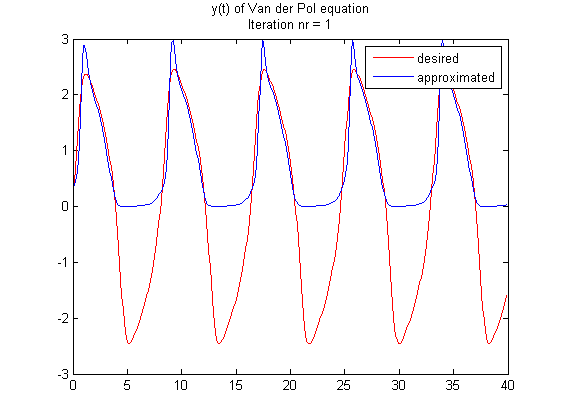
\includegraphics[width=0.5\textwidth]
	{images/signal_iter1.png}}
	\subfloat
	{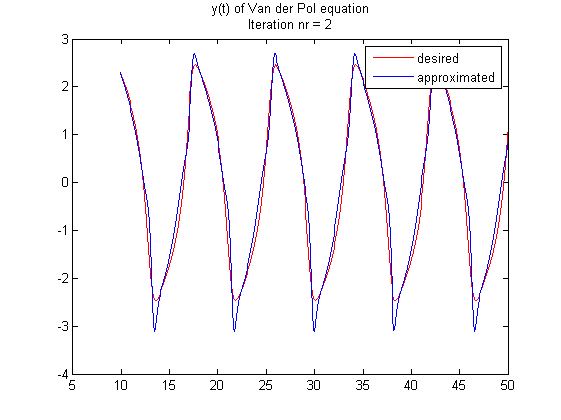
\includegraphics[width=0.5\textwidth]
	{images/signal_iter2.png}}
	
	\subfloat
	{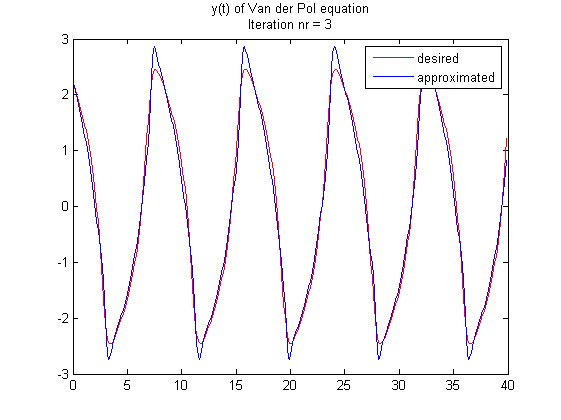
\includegraphics[width=0.5\textwidth]
	{images/signal_iter3.png}}
	\subfloat
	{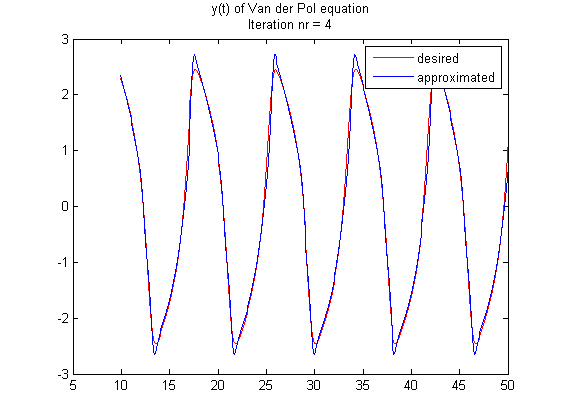
\includegraphics[width=0.5\textwidth]
	{images/signal_iter4.png}}

	\caption{Aproksymacja funkcji y(t) po selekcji funkcji numer 1-4}		
	\label{fig:signal_approx_a}		
\end{figure}

\begin{figure}[ht!]
	\centering

	\subfloat
	{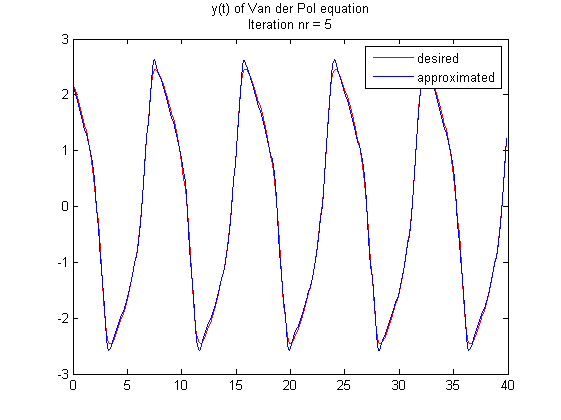
\includegraphics[width=0.5\textwidth]
	{images/signal_iter5.png}}
	\subfloat
	{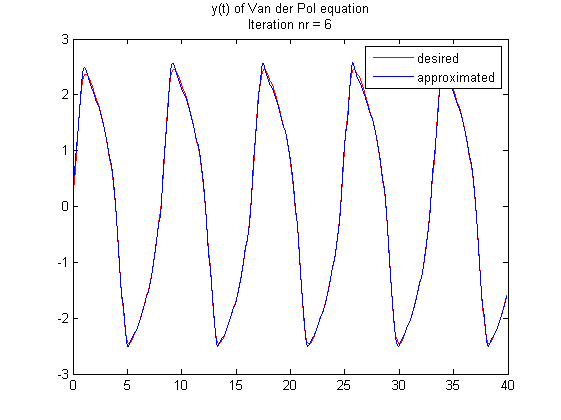
\includegraphics[width=0.5\textwidth]
	{images/signal_iter6.png}}	

	\caption{Aproksymacja funkcji y(t) po selekcji funkcji numer 5-6}		
	\label{fig:signal_approx_b}		
\end{figure}

\begin{figure}[ht!]
	\centering
	
	\subfloat
	{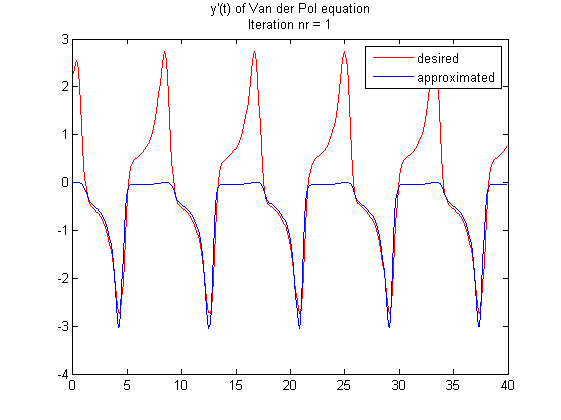
\includegraphics[width=0.5\textwidth]
	{images/deriv_iter1.png}}
	\subfloat
	{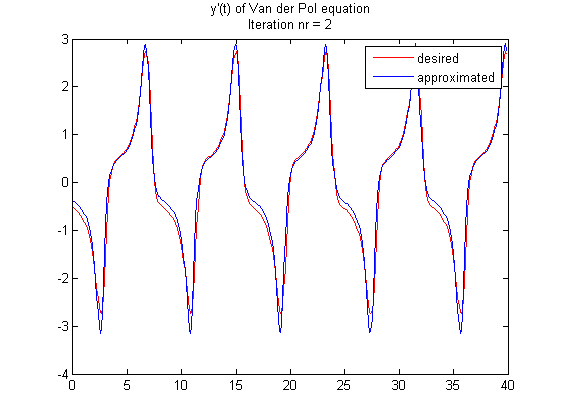
\includegraphics[width=0.5\textwidth]
	{images/deriv_iter2.png}}
	
	\subfloat
	{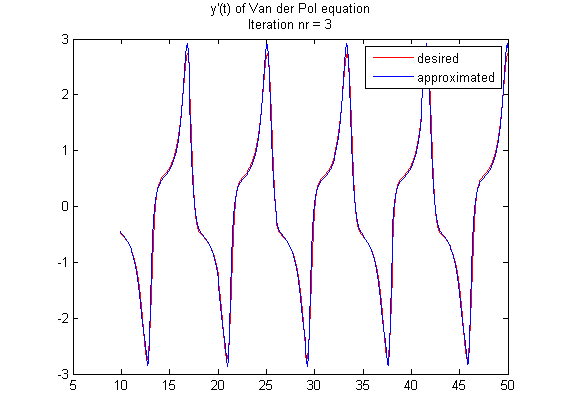
\includegraphics[width=0.5\textwidth]
	{images/deriv_iter3.png}}
	\subfloat
	{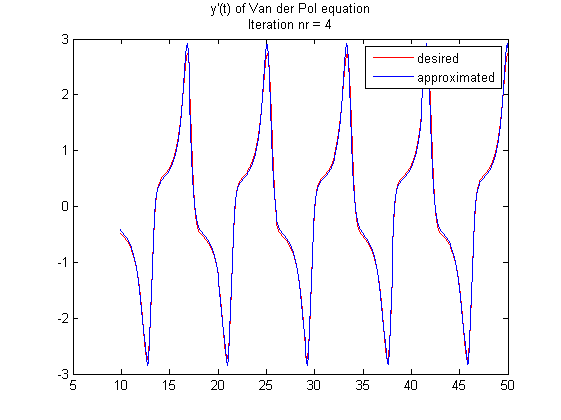
\includegraphics[width=0.5\textwidth]
	{images/deriv_iter4.png}}

	\caption{Aproksymacja funkcji y'(t)  po selekcji funkcji numer 1-4}		
	\label{fig:deriv_approx_a}
\end{figure}

\begin{figure}[ht!]
	\centering
	
	\subfloat
	{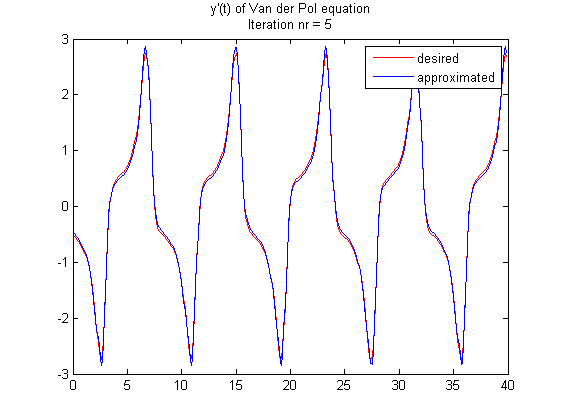
\includegraphics[width=0.5\textwidth]
	{images/deriv_iter5.png}}
	\subfloat
	{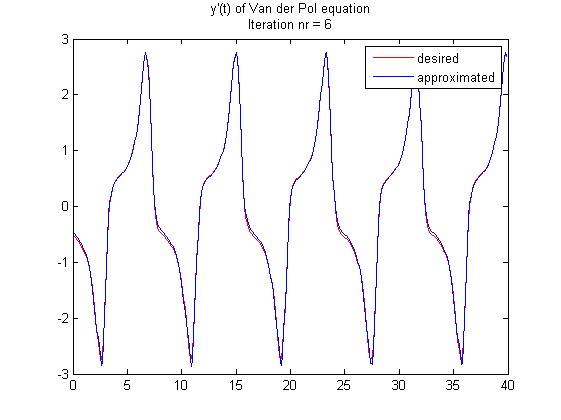
\includegraphics[width=0.5\textwidth]
	{images/deriv_iter6.png}}	
	
	\caption{Aproksymacja funkcji y'(t) po selekcji funkcji numer 5-6}		
	\label{fig:deriv_approx_b}
\end{figure}

Rysunek \ref{img:approximated} przedstawia aproksymację równania Van der Pola przez wytrenowaną sieć.

\begin{figure}[ht!]
	\centering

	\subfloat
	{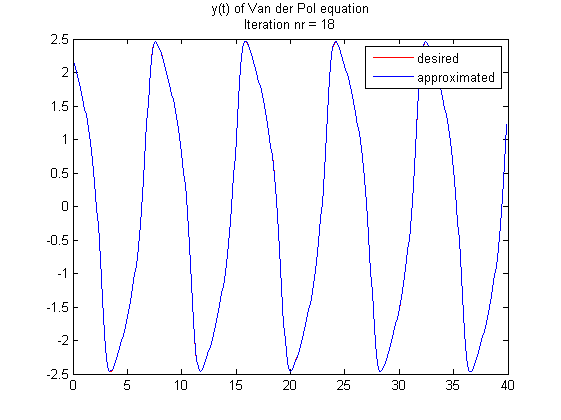
\includegraphics[width=0.5\textwidth]
	{images/signal_approx.png}}
	\subfloat
	{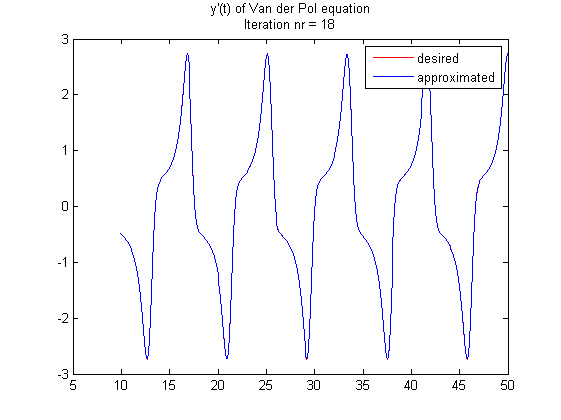
\includegraphics[width=0.5\textwidth]
	{images/deriv_approx.png}}	
	
	\subfloat
	{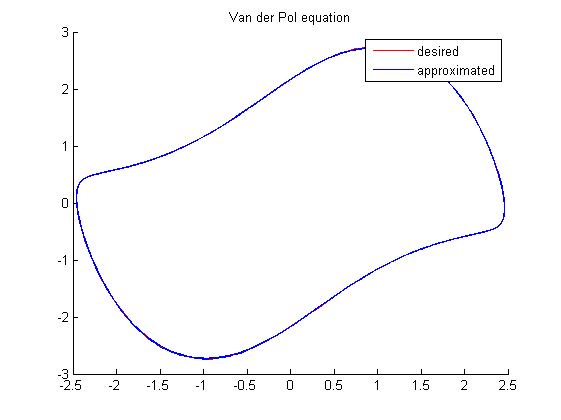
\includegraphics[width=0.5\textwidth]
	{images/trajectory_approx.png}}

	\caption{Sygnał zadany oraz aproksymowany przez wytrenowaną sieć RBF}
	\label{img:approximated}
\end{figure}


W tabeli \ref{tab:rbf_tabela_x1} zostały zebrane dane na temat wybranych funkcji RBF oraz błąd średniokwadratowy aproksymacji funkcji $y(t)$ równania Van der Pola po selekcji kolejnych funkcji RBF.
\begin{table}[ht!]
\centering

\begin{tabular}{ | c| c| c| c| c| c| c| }
\hline
number & indeks RBF & centrum 1 & centrum 2 & szerokość $\sigma$ & energia      & błąd MSE \\ \hline    	
  1 &  12  & -3.1502 &  -0.7340 &   1.5679  &  5.0151e-1 & 1.4482e+0 \\
  2 &   8  &  5.4297 &   0.9768 &   2.5525  &  4.6984e-1 & 8.3239e-2 \\
  3 &   2  & -7.7564 &  -1.6021 &   4.0418  &  1.6007e-2 & 3.6734e-2 \\
  4 &  98  &  2.2350 &  -3.0617 &   0.7123  &  6.0461e-3 & 1.9169e-2 \\
  5 &  29  &  1.0708 &   3.0705 &   1.0373  &  4.9545e-3 & 4.7753e-3 \\
  6 &   7  &  1.7366 &  -1.5238 &   1.9569  &  9.6330e-4 & 1.9766e-3 \\
  7 &   9  &  3.8691 &   3.7103 &   2.7734  &  4.2187e-4 & 7.5101e-4 \\
  8 &  92  &  1.1831 &  -0.3315 &   0.6019  &  1.3156e-4 & 3.6880e-4 \\
  9 &  10  & -3.2937 &  -2.9518 &   1.0999  &  8.6588e-5 & 1.1725e-4 \\
 10 &  94  &  1.4036 &   0.7138 &   0.6245  &  2.5108e-5 & 4.4300e-5 \\
 11 &  41  & -2.4064 &   1.1162 &   0.4944  &  4.6381e-6 & 3.0825e-5 \\
 12 &  87  &  0.7798 &   1.8971 &   0.4901  &  3.6228e-6 & 2.0300e-5 \\
 13 &  74  & -0.0576 &  -0.6049 &   0.5650  &  1.4344e-6 & 1.6133e-5 \\
 14 & 102  &  1.9120 &   0.0648 &   0.4207  &  2.1460e-6 & 9.8983e-6 \\
 15 &  33  &  2.6636 &   1.3395 &   1.1488  &  1.6053e-6 & 5.2345e-6 \\
 16 &  62  & -0.6188 &  -2.9390 &   0.5726  &  8.3324e-7 & 2.8137e-6 \\
 17 &  28  &  1.3729 &   1.3721 &   1.1716  &  4.7268e-7 & 1.4405e-6 \\
 18 &  73  &  0.0010 &  -1.3687 &   0.5821  &  1.6391e-7 & 9.6426e-7 \\
    \hline
\end{tabular}

\caption{Wybrane funkcje RBF dla y(t)}
\label{tab:rbf_tabela_x1}
\end{table}

\clearpage
W tabeli \ref{tab:rbf_tabela_x2} zostały zebrane dane na temat wybranych funkcji RBF oraz błąd średniokwadratowy aproksymacji pochodnej $y'(t)$ równania Van der Pola po selekcji kolejnych funkcji RBF.

\begin{table}[ht!]
\centering

\begin{tabular}{ |c| c| c| c| c| c| c| }
\hline
numer & indeks RBF & centrum 1 & centrum 2 & szerokość $\sigma$ & energia      & błąd MSE    \\ \hline    
  1 &  20 &   1.1473 &  -5.6855 &   2.0429 &   4.8617e-1 & 9.7778e-1 \\
  2 &  24 &  -0.6236 &   5.0850 &   2.1712 &   4.9394e-1 & 3.7858e-2 \\
  3 &  71 &   0.4130 &  -3.5541 &   0.8247 &   1.1341e-2 & 1.6276e-2 \\
  4 &  55 &  -1.4537 &  -1.3821 &   0.6111 &   4.7182e-3 & 7.2976e-3 \\
  5 & 105 &   2.8269 &   2.3932 &   0.7227 &   1.9348e-3 & 3.6158e-3 \\
  6 &  87 &   0.4346 &   2.4643 &   0.6928 &   9.1685e-4 & 1.8711e-3 \\
  7 &  31 &   2.7266 &  -1.5028 &   1.1935 &   5.1995e-4 & 8.8168e-4 \\
  8 &  35 &  -2.4119 &  -2.8131 &   0.4002 &   1.8068e-4 & 5.3787e-4 \\
  9 &  37 &  -3.3579 &  -1.5420 &   0.7055 &   8.9776e-5 & 3.6703e-4 \\
 10 &  62 &  -0.6019 &  -3.3353 &   0.4221 &   7.6543e-5 & 2.2138e-4 \\
 11 &  72 &  -0.0935 &  -1.9366 &   0.5978 &   2.3326e-5 & 1.7699e-4 \\
 12 &  34 &   2.2537 &   2.2456 &   1.0270 &   1.7366e-5 & 1.4394e-4 \\
 13 & 108 &   2.8131 &  -2.1200 &   0.5804 &   1.4160e-5 & 1.1700e-4 \\
 14 &  79 &   0.1034 &   2.5772 &   0.5442 &   2.3422e-5 & 7.2429e-5 \\
 15 &  46 &  -1.9263 &  -1.3252 &   0.5768 &   1.3428e-5 & 4.6876e-5 \\
 16 &  39 &  -3.6409 &   0.1476 &   0.7214 &   1.4115e-5 & 2.0016e-5 \\
 17 &   8 &   2.7340 &   0.0049 &   2.3398 &   4.4721e-6 & 1.1506e-5 \\
 18 &  73 &  -0.0732 &  -1.2943 &   0.5814 &   1.3090e-6 & 9.0150e-6 \\
 19 &  19 &  -1.5287 &   2.9209 &   1.1738 &   5.0646e-7 & 8.0513e-6 \\
 20 &  38 &  -2.8697 &  -0.7094 &   0.5993 &   2.7376e-7 & 7.5303e-6 \\
 21 &  44 &  -2.2676 &  -2.9283 &   0.5973 &   8.8402e-7 & 5.8481e-6 \\
 22 &  98 &   2.0550 &  -2.7400 &   0.5853 &   2.7736e-6 & 5.7016e-7 \\
    \hline
\end{tabular}


\caption{Wybrane funkcje RBF dla y'(t)}
\label{tab:rbf_tabela_x2}
\end{table}

\clearpage

Błąd średniokwadratowy w funkcji wybranych funkcji RBF przedstawia rysunek \ref{img:prediction_error} natomiast rysunek \ref{img:energy} przedstawia energię jaką wnosi każda kolejna wybrana funkcja. Jak można zauważyć główny wpływ na wartość błędu oraz energii mają dwie pierwsze wybrane funkcje. Wraz z wyborem kolejnych funkcji, błąd oraz energia wnoszona przez wybraną funkcję spadają w przybliżeniu logarytmicznie. Zieloną linią na wykresie \ref{img:prediction_error} została oznaczona wartość MSE, która jest warunkiem zakończenia uczenia sieci.

\begin{figure}[ht!]
	\centering

	{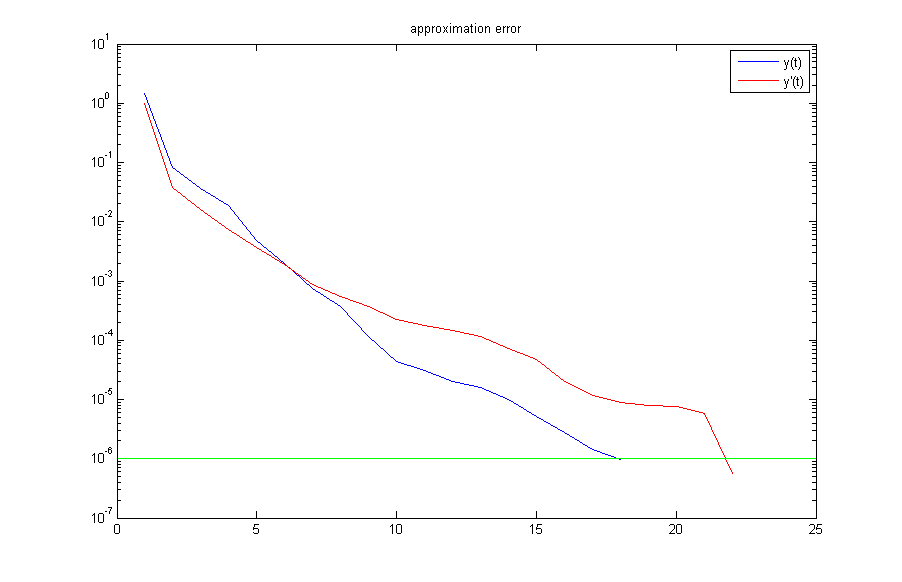
\includegraphics[width=\textwidth]
	{images/approximation_error.png}}

	\caption{Błąd MSE w funkcji wybranych funkcji RBF}
	\label{img:prediction_error}
\end{figure}


\begin{figure}[ht!]
	\centering

	{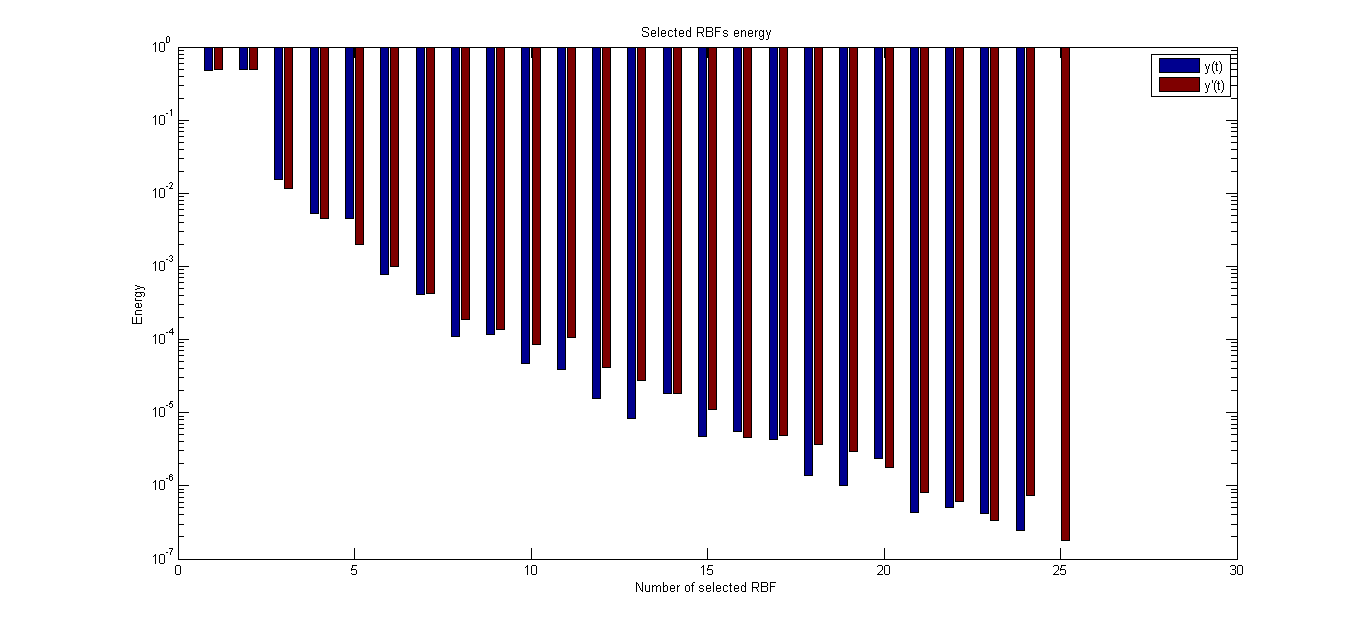
\includegraphics[width=0.8\textwidth]
	{images/rbfs_energy.png}}

	\caption{Energia wnoszona przez kolejne wybrane funkcji RBF}
	\label{img:energy}
\end{figure}

Po etapie trenowania sieci RBF sprawdzono jakość predykcji. Predykcja na 100 kroków do przodu została przedstawiona na rysunku~\ref{img:predicted}. Jak można zauważyć sieć dobrze modeluje obiekt opisany równaniem Van der Pola. Błąd średniokwadratowy dla wyznaczania $y(t)$ wyniósł  $1.6318e^{-3}$, natomiast błąd predykcji wyznaczania $y'(t)$ wyniósł $2.4210e^{-3}$.

\begin{figure}[ht!]
	\centering

	\subfloat
	{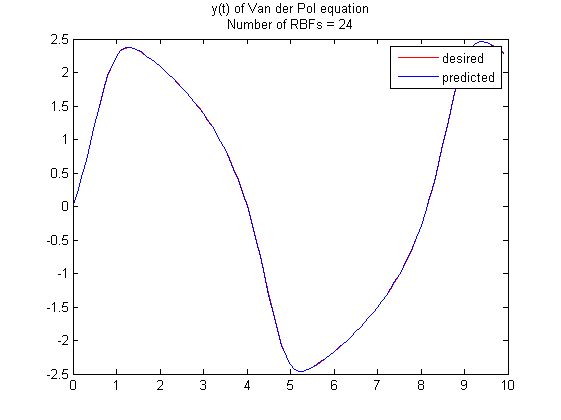
\includegraphics[width=0.45\textwidth]
	{images/signal_pred100.png}}
	\subfloat
	{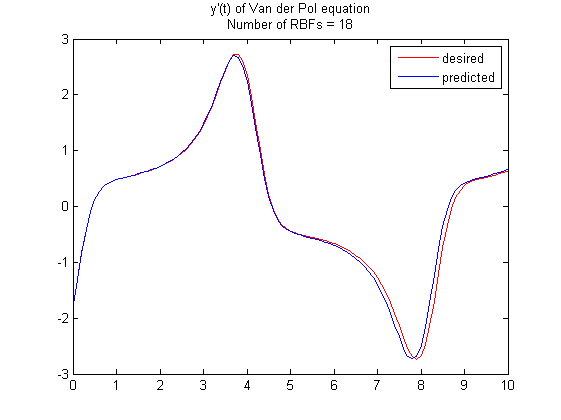
\includegraphics[width=0.45\textwidth]
	{images/deriv_pred100.png}}	
	
	\subfloat
	{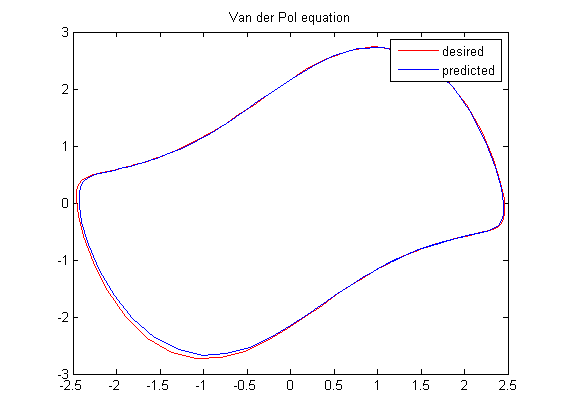
\includegraphics[width=0.45\textwidth]
	{images/trajectory_pred100.png}}

	\caption{Sygnał zadany oraz przewidywany przez wytrenowaną sieć RBF $t \in [0,10]$}
	\label{img:predicted}
\end{figure}

Trudno jest jednak dokładniej określić jakość predykcji na podstawie rysunku \ref{img:predicted} ze względu na nieznaczne różnice w wartości zadanej oraz wartości przewidywanej przez sieć w wyniku czego sygnał zadany oraz przewidywany pokrywają się. Aby można było dokładnie określić odstępstwo wartości przewidywanej od wartości rzeczywistej na rysunku \ref{img:err100_x} został przedstawiony błąd predykcji w kolejnych krokach. Wartość bezwzględna błędu wyznaczenia $y(t)$ nie przekracza wartości 0.09, natomiast maksymalny błąd wyznaczenia $y'(t)$ nie przekracza wartości 0.16. Na tej podstawie można stwierdzić, że dla 100 kroków w przód sieć spełnia swoje zadanie. 

\begin{figure}[ht!]
	\centering

	\subfloat
	{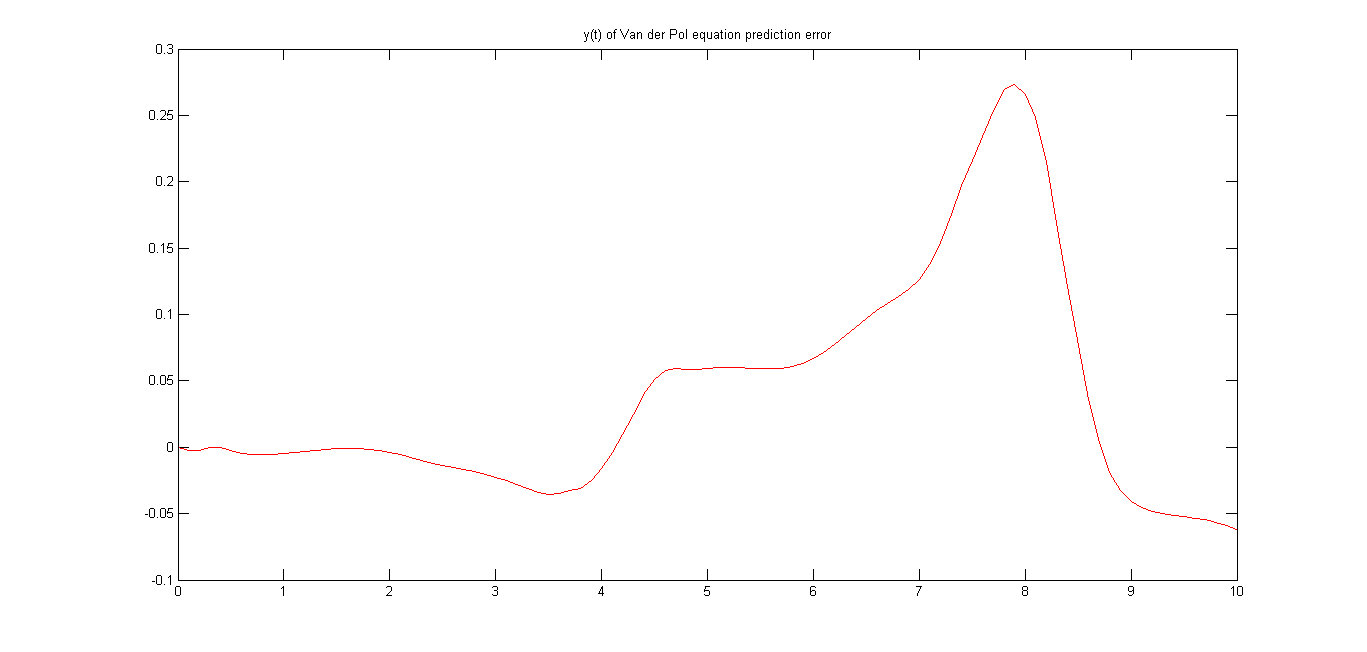
\includegraphics[width=0.5\textwidth]
	{images/err100_x1.png}}
	\subfloat
	{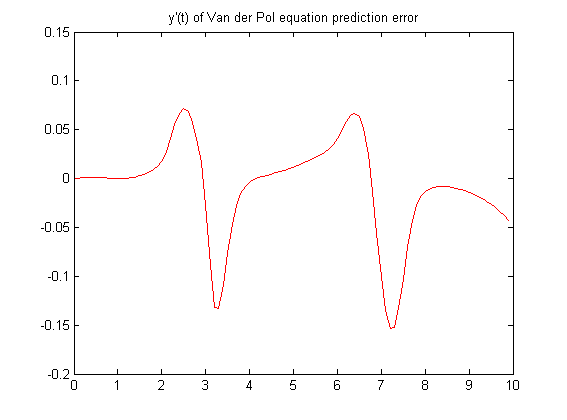
\includegraphics[width=0.5\textwidth]
	{images/err100_x2.png}}	
	

	\caption{Błąd predykcji w funkcji czasu $t \in [0,10]$}
	\label{img:err100_x}
\end{figure}


Następnie zdecydowano się na sprawdzenie jakości predykcji w 5-krotnie dłuższym przedziale czasu $t \in [0, 50]$. Na rysunku \ref{img:predicted2} został przedstawiany sygnał rzeczywisty oraz przewidywany. Jak można zauważyć wraz z oddalaniem się od punktu początkowego charakterystyki zadana oraz przewidywana rozbiegają się. Błąd średniokwadratowy dla wyznaczania $y(t)$ wyniósł  0.0754, natomiast błąd wyznaczania $y'(t)$ wyniósł 0.1187, czyli kilkukrotnie wzrósł w stosunku do błędu dla 5-kronie krótszego okresu predykcji.

\begin{figure}[ht!]
	\centering

	\subfloat
	{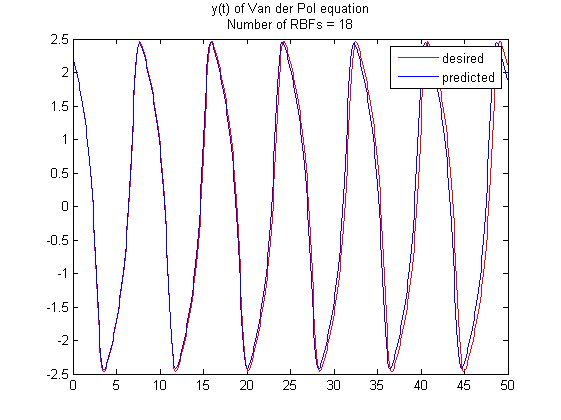
\includegraphics[width=0.5\textwidth]
	{images/signal_pred400.png}}
	\subfloat
	{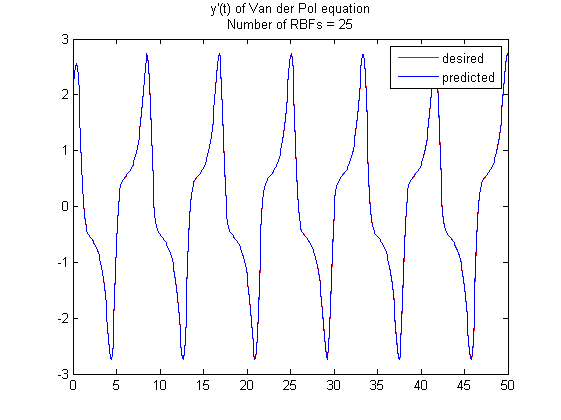
\includegraphics[width=0.5\textwidth]
	{images/deriv_pred400.png}}	
	
	\subfloat
	{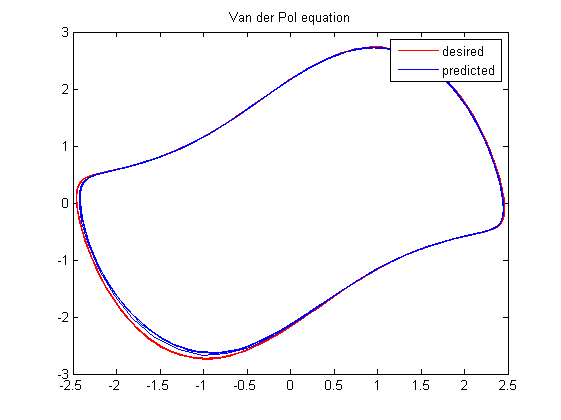
\includegraphics[width=0.5\textwidth]
	{images/trajectory_pred400.png}}

	\caption{Sygnał zadany oraz przewidywany przez wytrenowaną sieć RBF $t \in [0,50]$}
	\label{img:predicted2}
\end{figure}

Aby dokładniej określić jakość predykcji w przedziale czasu $t \in [0, 50]$ ponownie skorzystano z wykresu błędu predykcji dla kolejnych kroków. Jak można zauważyć wraz z oddalaniem się od punktu początkowego błąd predykcji rośnie. Dzieje się tak ze względu na akumulację błędu. Po 500 krokach różnice wartości zadanej i przewidywanej są już znaczne co wyklucza możliwość właściwej predykcji dla tak długiego okresu czasu.

\begin{figure}[ht!]
	\centering

	\subfloat
	{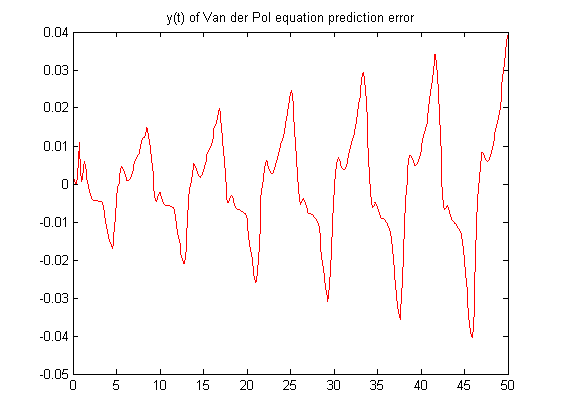
\includegraphics[width=0.5\textwidth]
	{images/err1000_x1.png}}
	\subfloat
	{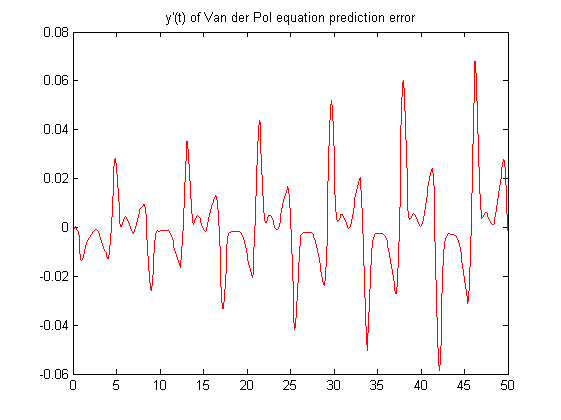
\includegraphics[width=0.5\textwidth]
	{images/err1000_x2.png}}	
	

	\caption{Błąd predykcji w funkcji czasu $t \in [0,50]$}
	\label{img:err}
\end{figure}

Do tej pory badana była jedynie predykcja dla tych samych warunków początkowych dla jakich sieć została wytrenowana. Jednak aby model był dobrze odwzorowany należałoby sprawdzić czy sieć jest zdolna do predykcji dla szerszego zakresu warunków początkowych. W tym celu została przeprowadzona predykcja dla 440 różnych wartości początkowych równomiernie rozłożonych w przestrzeni $[-2,2] \times [-2,2]$ dla 100 kroków w przód. Jakość predykcji została oceniona na podstawie błędu średniokwadratowego. Wykres obrazujący jakość predykcji w~zależności od warunków początkowych przedstawia rysunek \ref{img:err_initial}.

\begin{figure}[ht!]
	\centering

	\subfloat[y(t)]
	{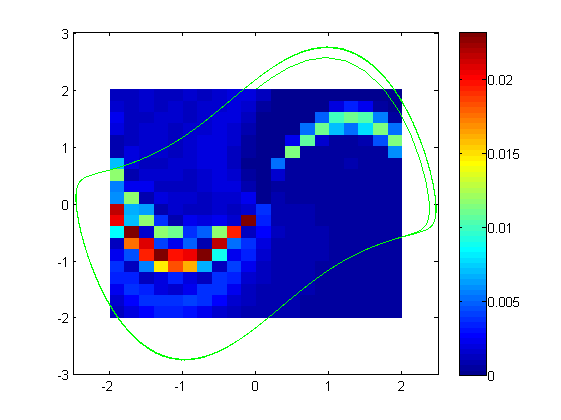
\includegraphics[width=0.5\textwidth]
	{images/figure_signal.png}}
	\subfloat[y'(t)]
	{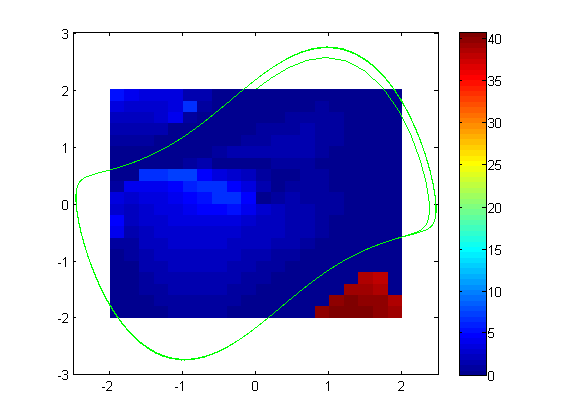
\includegraphics[width=0.5\textwidth]
	{images/figure_deriv.png}}	
	

	\caption{Błąd predykcji w zależności od warunków początkowych $t \in [0,10]$}
	\label{img:err_initial}
\end{figure}

Sieć dobrze modeluje obiekt dla większości warunków początkowych. Ustalając akceptowalność predykcji, dla której błąd MSE był mniejszy niż 0.01, sieć była w stanie poprawnie modelować obiekt dla 402 z 440 warunków początkowych. Stworzony model zatem jest odpowiedni dla właściwego zbioru warunków początkowych. Aby sieć neuronowa była w stanie modelować równanie w szerszym zakresie warunków początkowych zwiększono wielkość zbioru uczącego. W tym celu rozwiązano równanie Van der Pola dla tych samych warunków początkowych co poprzednio w przedziale dziesięciokrotnie dłuższym $t \in [0,500]$.

Osiągnięcie błędu średniokwadratowego poniżej $1e^{-6}$ udało się osiągnąć dla 15 funkcji bazowych dla funkcji $y(t)$ (błąd równy $9.8312e^{-7}$) oraz 26 funkcji bazowych dla pochodnej $y'(t)$ (błąd równy = $6.5825e^{-7}$).

\clearpage
W tabeli \ref{tab:rbf_tabela2_x1} zostały zebrane dane na temat wybranych funkcji RBF oraz błąd średniokwadratowy aproksymacji $y(t)$ po selekcji kolejnych funkcji RBF.

\begin{table}[ht!]
\centering

\begin{tabular}{ |c| c| c| c| c| c| c| }
\hline
numer & indeks RBF & centrum 1 & centrum 2 & szerokość $\sigma$ & energia      & błąd MSE    \\ \hline    
    1 &  32 &   3.0688  &  0.7251  &  1.5408  &  4.7435e-1 & 1.5650e+0 \\
    2 &   2 &  -5.8240  & -1.0400  &  2.6736  &  4.9778e-1 & 8.3000e-2 \\
    3 &   8 &   8.7131  &  1.7688  &  4.2841  &  1.5672e-2 & 3.6341e-2 \\
    4 &  52 &  -2.2450  &  3.0386  &  0.7082  &  5.8876e-3 & 1.8812e-2 \\
    5 &  15 &  -1.0732  & -3.0634  &  1.0248  &  4.7462e-3 & 4.6817e-3 \\
    6 &   3 &  -1.8519  &  1.6768  &  2.0134  &  9.2030e-4 & 1.9418e-3 \\
    7 &   1 &  -3.3016  & -3.1929  &  2.5308  &  4.4272e-4 & 6.2367e-4 \\
    8 & 101 &   2.3115  & -0.8549  &  0.6729  &  1.2278e-4 & 2.5812e-4 \\
    9 &  40 &  -2.6310  &  0.6152  &  0.4777  &  4.4630e-5 & 1.2524e-4 \\
   10 &  10 &  -3.2870  & -3.2361  &  1.3004  &  3.0012e-5 & 3.5891e-5 \\
   11 &  97 &   1.2062  &  2.4778  &  0.4767  &  6.6179e-6 & 1.6187e-5 \\
   12 &  89 &   1.3713  & -2.8097  &  0.5886  &  3.8504e-6 & 4.7238e-6 \\
   13 &  85 &   0.7152  &  0.7106  &  0.5556  &  9.1151e-7 & 2.0100e-6 \\
   14 &  34 &   3.2081  &  3.0810  &  1.2494  &  1.8630e-7 & 1.4554e-6 \\
   15 &  74 &   0.0057  & -0.6810  &  0.5077  &  1.5862e-7 & 9.8312e-7 \\
\hline
\end{tabular}

\caption{Wybrane funkcje RBF dla y(t)}
\label{tab:rbf_tabela2_x1}
\end{table}

\clearpage
W tabeli \ref{tab:rbf_tabela2_x2} zostały zebrane dane na temat wybranych funkcji RBF oraz błąd średniokwadratowy aproksymacji $y'(t)$ po selekcji kolejnych funkcji RBF.

\begin{table}[ht!]
\centering

\begin{tabular}{ |c| c| c| c| c| c| c| }
\hline
numer & indeks RBF & centrum 1 & centrum 2 & szerokość $\sigma$ & energia      & błąd MSE    \\ \hline    
  1 &  20  &  1.0045 &  -5.3066  &  1.9706 &   4.7630e-1 & 9.8356e-1  \\
  2 &  24  & -0.6017 &   5.1099  &  2.1817 &   5.0336e-1 & 3.8203e-2  \\
  3 &  71  &  0.4205 &  -3.4722  &  0.8295 &   1.1804e-2 & 1.6034e-2  \\
  4 &  55  & -1.3286 &  -1.3163  &  0.5824 &   4.1755e-3 & 8.1916e-3  \\
  5 & 105  &  2.8304 &   2.3903  &  0.7111 &   2.0601e-3 & 4.3224e-3  \\
  6 &  18  & -1.7754 &   2.0452  &  0.8914 &   1.0196e-3 & 2.4076e-3  \\
  7 &  31  &  2.9322 &  -1.5813  &  1.0904 &   6.3660e-4 & 1.2120e-3  \\
  8 &  35  & -2.4503 &  -2.8244  &  0.4318 &   2.1830e-4 & 8.0199e-4  \\
  9 &  34  &  3.4515 &   3.3322  &  1.2735 &   1.4452e-4 & 5.3057e-4  \\
 10 &  51  & -2.0114 &   1.9973  &  0.5857 &   7.2852e-5 & 3.9375e-4  \\
 11 &   4  &  0.0131 &  -2.5200  &  2.2110 &   7.9188e-5 & 2.4502e-4  \\
 12 &  52  & -2.1064 &   2.8180  &  0.5952 &   3.1678e-5 & 1.8553e-4  \\
 13 &  44  & -2.2926 &  -2.9826  &  0.6061 &   4.9411e-5 & 9.2731e-5  \\
 14 &  95  &  1.3808 &   1.3767  &  0.5865 &   1.4960e-5 & 6.4635e-5  \\
 15 & 108  &  2.6828 &  -1.9563  &  0.5559 &   1.4746e-5 & 3.6940e-5  \\
 16 &  59  & -1.2458 &   1.2003  &  0.6075 &   1.2079e-5 & 1.4255e-5  \\
 17 &   5  & -0.0010 &  -0.0005  &  2.3399 &   1.2461e-6 & 1.1914e-5  \\
 18 &  37  & -2.6619 &  -1.3051  &  0.5671 &   9.9185e-7 & 1.0052e-5  \\
 19 &  57  & -1.4292 &   0.0738  &  0.5893 &   1.1842e-6 & 7.8277e-6  \\
 20 &  46  & -2.0750 &  -1.3772  &  0.5875 &   1.9370e-6 & 4.1898e-6  \\
 21 &  16  & -1.3775 &  -1.3752  &  1.1747 &   7.4375e-7 & 2.7930e-6  \\
 22 &  85  &  0.6860 &   0.6869  &  0.5887 &   5.5876e-7 & 1.7435e-6  \\
 23 &  87  &  0.6914 &   2.0588  &  0.5738 &   1.8307e-7 & 1.3997e-6  \\
 24 &  38  & -2.6860 &  -0.6726  &  0.5734 &   9.5668e-8 & 1.2200e-6  \\
 25 &  30  &  2.7394 &  -2.7394  &  1.1720 &   1.1646e-7 & 1.0013e-6  \\
 26 &  83  &  0.6805 &  -0.6899  &  0.5908 &   1.8267e-7 & 6.5825e-7  \\
   \hline
\end{tabular}

\caption{Wybrane funkcje RBF dla y'(t)}
\label{tab:rbf_tabela2_x2}
\end{table}

\clearpage
 Następnie sprawdzono czy sieć po zwiększeniu zbioru uczącego jest w stanie lepiej modelować układ dla różnych warunków początkowych. Wykres obrazujący jakość predykcji w zależności od warunków początkowych przedstawia rysunek \ref{img:err_initial2}.


\begin{figure}[ht!]
	\centering

	\subfloat[y(t)]
	{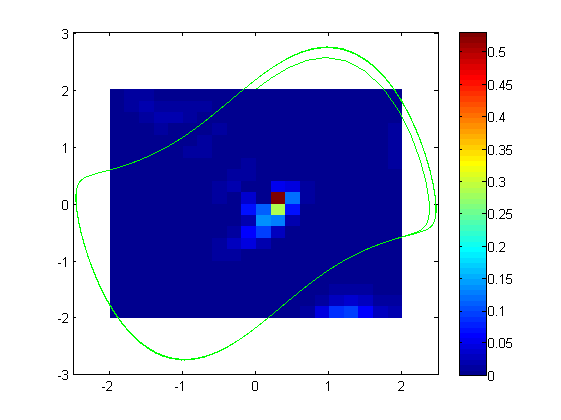
\includegraphics[width=0.5\textwidth]
	{images/figure_signal2.png}}
	\subfloat[y'(t)]
	{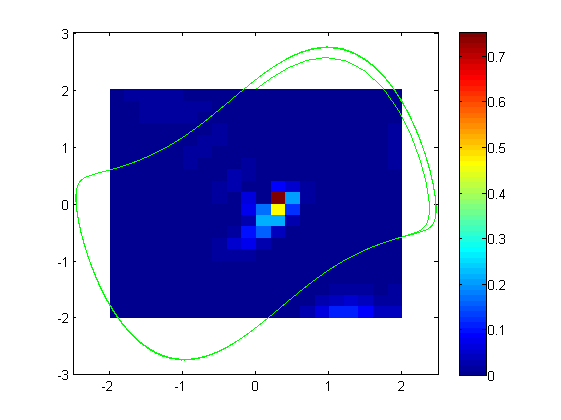
\includegraphics[width=0.5\textwidth]
	{images/figure_deriv2.png}}	
	

	\caption{Błąd predykcji w zależności od warunków początkowych $t \in [0,10]$}
	\label{img:err_initial2}
\end{figure}

Zakładając akceptowalność predykcji na takim samym poziomie jak poprzednio (MSE $<$ 0.01) sieć dobrze modeluje układ dla wszystkich warunków początkowych. Największa wartość błędu wynosiła odpowiednio $1.8703e^{-4}$ dla $y(t)$ oraz  $3.3520e^{-4}$ dla $y'(t)$. W porównaniu do wartości maksymalnej wartości błędu dla sieci uczonej na podstawie danych z trajektorii w przedziale $t \in [0,50]$ (maksymalny błąd MSE dla $y(t)$ wynosił $2.3169e^{-2}$, natomiast dla $y'(t)$ wynosił $3.2620e^{-2}$) błąd średniokwadratowy zmalał ponad kilkadziesiąt krotnie.

\clearpage
\section{Podsumowanie oraz wnioski}

Celem pracy była próba identyfikacji nieliniowych obiektów dynamicznych z wykorzystaniem metody GOFR. Cel udało się zrealizować na przykładzie obiektu dynamicznego opisanego równaniem Van der Pola. Posiadając dane tylko z jednej trajektorii sieć była w stanie dobrze modelować obiekt dla różnych warunków początkowych. Predykcja na 100 kroków w przód skutkowała błędem średniokwadratowym aproksymacji $y(t)$ równym $1.6318e^{-3}$ oraz błędem aproksymacji $y'(t)$ równym $2.4210e^{-3}$. Następnie zwiększono wielkość zbioru danych uczących 10-krotnie. Po ponownym wytrenowaniu sieci okazało się, że jakość aproksymacji modelu dla uległa znacznemu polepszeniu.
Określając jako akceptowalną predykcje taką, dla której błąd MSE $<$ 0.01 dla $y(t)$ oraz $y'(t)$ jednocześnie, udało się uzyskać poprawną predykcję dla wszystkich warunków początkowych.

Czas uczenia sieci uległ jednak znacznemu wydłużeniu. Liczba funkcji bazowych zwiększyła się nieznacznie z 40 do 41. Jednym z ograniczeń zaproponowanej metody identyfikacji jest modelowanie obiektu dla z góry określonego kroku (dla identyfikowanego obiektu h = 0.1). Rozwiązanie takiego problemu zostało jednak zaproponowane w pracy Yi-Jen Wanga i Chin-Teng Lina\cite{Wang}. Wykorzystane w tym celu zostało połączenie metody Runge-Kutty oraz radialnej sieci neuronowej. Sieć przedstawioną w pracy można wykorzystać w tej metodzie tak aby umożliwić swobodny dobór kroku metody.

W pracy \cite{Masri} została podjęta próba identyfikacji dynamiki obiektu opisanego równaniem Van der Pola z wykorzystaniem perceptronu wielowarstwowego. Oceniając jakościowo identyfikację obiektu z wykorzystaniem perceptronu wielowarstwowego można stwierdzić, że zaproponowana w pracy dyplomowej metoda pozwoliła uzyskać lepsze wyniki.

Przedstawiona w pracy metoda sprawdziła się w identyfikacji dynamiki obiektu nieliniowego opisanego równaniem Van der Pola. W dalszych pracach można wykorzystać metodę GOFR do identyfikacji innych nieliniowych obiektów dynamicznych oraz zastosować ją w połączeniu z metodą Runge-Kutty\cite{Wang}.

Program został zaimplementowany z użyciem języka programowania MATLAB. Listingi kodu źródłowego zostały zamieszone w Dodatku A.

% -------------------------- bibliografia ----------------------------
\clearpage

\addcontentsline{toc}{section}{Literatura}
\begin{thebibliography}{widest-label}

\bibitem{Bartkowiak} Bartkowiak A., Sieci RBF - o radialnych funkcjach bazowych (popr. 05.12.2009 i 14.12.2010), \url{https://www.ii.uni.wroc.pl/~aba/teach/NN/w9rbf.pdf}

\bibitem{Bernardelli} Michał Bernardelli, Wprowadzenie do Metod Numerycznych -
Zajęcia nr 6, 9 listopada 2011, \url{http://akson.sgh.waw.pl/~mbernard/Dydaktyka/Rok\_2010\_11/WprowadzenieD oMetodNumerycznychLic\_1011\_let/Zajecia06.pdf}

\bibitem{Bishop}Bishop C. M., Neural Networks for Pattern Recognition, Oxford University Press, Oxford 1995 

\bibitem{Bors} A. G. Bors, Introduction of the Radial Basis Function (RBF) Networks, Online Symposium for Electronics Engineers, issue 1, vol. 1, DSP Algorithms: Multimedia, Feb. 13 2001, pp. 1-7. 

\bibitem{Chen} Chen S., Cowan C. F. N., Grant P. M., Orthogonal Least Squares Learning Algorithm for Radial Basis Function Networks, IEEE Transaction on Neural Networks, vol 2, no. 2, p. 302-309, 1991

\bibitem{BCh_2001} Choczewski B. (red.), Równania różniczkowe zwyczajne i cząstkowe. Zadania z matematyki, Wydawnictwa AGH, Kraków 2001

\bibitem{Czemplik} Czemplik. A, Modele dynamiki układów fizycznych dla inżynierów
Zasady i przykłady konstrukcji modeli dynamicznych obiektów automatyki, WNT, Warszawa 2008

\bibitem{Osowski}Osowski S., Sieci neuronowe do przetwarzania informacji, Oficyna Wydawnicza Politechniki Warszawskiej,  Warszawa 2006

\bibitem{Duboisa} R. Dubois, B. Quenet, Y. Faisandier, G. Dreyfus, Building meaningful representations for nonlinear modeling of 1d- and 2d-signals: applications to biomedical signals, Neurocomputing 69 (2006), p. 2180–2192

\bibitem{Gutenbaum} J. Gutenbaum, Modelowanie systemów, Akademicka Oficyna Wydawnicza EXIT, Warszawa 2003

\bibitem{Isermann} Rolf Isermann, Marco Münchhof, Identification of Dynamic Systems: An Introduction with Applications, Springer, New York 2010

\bibitem{Jankowski} S. Jankowski, Szkic materiałów do wykładu: Sieci neuronowe i neurokomputery, Instytut Systemów Elektronicznych,
Politechnika Warszawska, Warszawa 2011

\bibitem{AK_RBG2002} A. Kharab, R. B. Guenther, An introduction to numerical methods : A MATLAB Approach, Chapman \& Hall, New York 2002

\bibitem{Kosinski} R. A. Kosiński, Sztuczne sieci neuronowe – dynamika nieliniowa i chaos, wyd. 3 uakt., WNT, Warszawa 2007

\bibitem{Masri} S. F. Masri, A. G. Chassiakos, T. K. Caughey, Structure-unknown non-linear dynamic systems: identification through neural networks, Smart Materials ans Structures 1 (1992), 45-56

\bibitem{Palczewski} Palczewski A., Równania różniczkowe zwyczajne
Teoria i metody numeryczne z wykorzystaniem komputerowego systemu obliczeń symbolicznych. Wyd. 2, WNT, Warszawa 2004

\bibitem{Tsatsos} Marios Tsatsos, Dissertation: Theoretical and Numerical Study of the Van der Pol equation, Aristotle University of Thessaloniki School of Sciences, , Thessaloniki July 2006

\bibitem{Wang} Yi-Jen Wang, Chin-Teng Lin, Runge–Kutta Neural Network for Identification of Dynamical Systems in High Accuracy, IEEE Transaction on Neural Networks, vol. 9, no. 2, march 1998

\end{thebibliography}

\clearpage
\addcontentsline{toc}{section}{Dodatek A: Kod źródłowy programu}
\section*{Dodatek A: Kod źródłowy programu}

\textbf{rk\_van\_der\_pol.m}

\begin{lstlisting}
% Function solving Van der Pol equations usign 4-th order Runge-Kutta method
%
% t_end - end of time period for solution (time starts from 0)
% h     - time step
% y0    - init values

function [t,y] = rk_van_der_pol(t_end, h, y0)
    % Runge-Kutta general formula
    % y_{i+1} = y_i + 1/6*(k_1 + 2k_2 + 2k_3 + k_4), i = 0,1,2,...
    % k_1 = hf(x_i,y_1)
    % k_2 = hf(x_i + 1/2h, y_1 + 1/2k_1)
    % k_3 = hf(x_i + 1/2h, y_1 + 1/2k_2)    
    % k_4 = hf(x_i + h, y_1 + k_3)
    
    t = 0:h:t_end;
    n = length(t);
    h = 0.1;

    y = zeros(n, 2);
    y(1, 1) = y0(1);
    y(1, 2) = y0(2);
    
    % Van der Pol equation 
    % y''(t) - (1 - y^2(t)) * y'(t) + y(t) = 0;
    % y'(t)  = y(2)
    % y''(t) = (1-y(1)^2)*y(2)-y(1)
    for i = 1:n-1
        k1 = h*(y(i,2));
        k2 = h*(y(i,2)+0.5*k1);
        k3 = h*(y(i,2)+0.5*k2);
        k4 = h*(y(i,2)+k3);
        y(i+1,1) = y(i,1)+(k1+2*k2+2*k3+k4)/6;
        
        y1 = y(i,1);
        y2 = y(i,2);
        k1 = h*((1-y1^2)*y2-y1);
        y1 = y(i,1)+0.5*k1;
        y2 = y(i,2)+0.5*k1;
        k2 = h*((1-y1^2)*y2-y1);
        y1 = y(i,1)+0.5*k2;
        y2 = y(i,2)+0.5*k2;
        k3 = h*((1-y1^2)*y2-y1);
        y1 = y(i,1)+k3;
        y2 = y(i,2)+k3;
        k4 = h*((1-y1^2)*y2-y1);
        y(i+1,2) = y(i,2)+(k1+2*k2+2*k3+k4)/6;
    end
end

\end{lstlisting}

\textbf{gofr.m}

\begin{lstlisting}
function [selected_rbfs, W, E_k, A_k, Q_k, B_k, centers, sigmas, G] =  gofr(X, y, G, centers, sigmas, K)

    rbf_number = length(centers);

    D = y;
    Q = zeros(size(G));
    Q_k = zeros(size(G));
    B = zeros(1,rbf_number);
    B_k = zeros(1,rbf_number);
    E = zeros(1,rbf_number);
    E_k = zeros(1,K);
    selected_rbfs = zeros(1,rbf_number);      % indexes of selected rbfs order by decreasing energy 

    A = cell(1,rbf_number);
    A_k = eye(rbf_number);
    for i = 1:rbf_number
        A{i} = eye(rbf_number);
    end

    % ----- selection of the most significant functions -----
    for k = 1:K
        % Gram-Schmidt orthogonalization
        for i = 1:rbf_number
           Q(:,i) = G(:,i);

           % if rbf is already selected function omit it 
           if ismember(i, selected_rbfs) == 1
               continue;
           end

           for j=1:k-1
                A{i}(j,k) = Q_k(:,j)'*G(:,i) / (Q_k(:,j)'*Q_k(:,j));
                Q(:,i) = Q(:,i) - A{i}(j,k)*Q_k(:,j);
           end

           B(i) = Q(:,i)'*D / (Q(:,i)'*Q(:,i));
           E(i) = B(i)^2*Q(:,i)'*Q(:,i) / (D'*D);   
        end

        % find RBF with maximum energy (save index and copy to Q_k matrix)
        [E_k(k) selected_rbfs(k)] = max(E);
        B_k(k) = B(selected_rbfs(k));
        A_k(:,k) = A{selected_rbfs(k)}(:,k);
        W = A_k\B_k';

        % ------ Levenberg-Marquardt -----
        Theta = [W(k); sigmas(selected_rbfs(k)); centers(1, selected_rbfs(k)); centers(2, selected_rbfs(k))];

        y_rbf = 0;
        for j = 1:k
            y_rbf = y_rbf + W(j) * gaussian_2D(X, sigmas(selected_rbfs(j)), centers(:,selected_rbfs(j))');
        end
        
        lambda = 0.1;
        Theta_old = Theta;
        N = 100;   % maximum iterations of gradient method
        err = zeros(N,1);
        err(1) = abs(sum((y - y_rbf).^2)) / length(y);
        err_old = err(1);
        for n = 2:N
            dy_dw = gaussian_2d(X, Theta(2), [Theta(3) Theta(4)]);
            dy_dsigma = Theta(1) * ((Theta(3) - X(:,1)).^2 + (Theta(4) - X(:,2)).^2) ./ (Theta(2)^3) .* gaussian_2d(X, Theta(2), [Theta(3) Theta(4)]);
            dy_dc1 = (Theta(1)*(X(:,1) - Theta(3))) ./ (Theta(2)^2) .* gaussian_2d(X, Theta(2), [Theta(3) Theta(4)]);
            dy_dc2 = (Theta(1)*(X(:,2) - Theta(4))) ./ (Theta(2)^2) .* gaussian_2d(X, Theta(2), [Theta(3) Theta(4)]);
            
            Z = [dy_dw dy_dsigma dy_dc1 dy_dc2];
            e = y - y_rbf;

            Theta = Theta + pinv(Z'*Z + lambda*eye(4))*Z'*e;            
            W(k) = Theta(1);
            sigmas(selected_rbfs(k)) = Theta(2);
            centers(1,selected_rbfs(k)) = Theta(3);
            centers(2,selected_rbfs(k)) = Theta(4);
            
            y_rbf = 0;
            for j = 1:k
                y_rbf = y_rbf + W(j) * gaussian_2D(X, sigmas(selected_rbfs(j)), centers(:,selected_rbfs(j))');
            end

            err(n) = sum((y - y_rbf).^2) / length(y);
            if (err(n) >= err_old)
                Theta = Theta_old;
                lambda = lambda * 10;
            else
                Theta_old = Theta;
                err_old = err(n);
                lambda = lambda / 10;                
            end

            % if lambda is too big or too small stop
            if (lambda > 1e6 || lambda < 1e-6)
                break;
            end;
            
            if (err(n) < 1e-6)
                break;
            end
        end;
        
        % set the optimal parameters
        W(k) = Theta_old(1);
        sigmas(selected_rbfs(k)) = Theta_old(2);
        centers(1,selected_rbfs(k)) = Theta_old(3);
        centers(2,selected_rbfs(k)) = Theta_old(4);

        % Gram-Schmidt orthogonalization for modified RBF
        i = selected_rbfs(k);
        G(:,i) = gaussian_2D(X, Theta(2), [Theta(3) Theta(4)]);
        Q(:,i) = G(:,i);

        for j=1:k-1
            A{i}(j,k) = Q_k(:,j)'*G(:,i) / (Q_k(:,j)'*Q_k(:,j));
            Q(:,i) = Q(:,i) - A{i}(j,k)*Q_k(:,j);
        end

        B(i) = Q(:,i)'*D / (Q(:,i)'*Q(:,i));
        B_k(k) = B(i);
        E_k(k) = B(i)^2*Q(:,i)'*Q(:,i) / (D'*D);
        A_k(:,k) = A{i}(:,k);
        Q_k(:,k) = Q(:,i);
        W = A_k\B_k';
        E = zeros(size(E));
    end

    W = A_k\B_k';
end
\end{lstlisting}

\textbf{generate\_library\_2d.m}

\begin{lstlisting}
% ----- Function generating radial basis function set -----
% N - number of dividing set iteration - change this variable if want other number of RBFs
% G - matrix with values of all rbf functions
% centers - vector of centers of all rbf functions
% sigmas - vector of sigma of all rbf functions
function [G,centers,sigmas] = generate_library_2d(X, N)

    rbf_number = 0; % total number of RBFs

    for i = 1:N
        rbf_number = rbf_number + (2^i + 1)^2;
    end

    G = zeros(length(X), rbf_number);
    centers = zeros(2, rbf_number);
    sigmas = zeros(1, rbf_number);
    k = 1;

    max_x = max(max(X));
    min_x = min(min(X));

    for i = 1:N

        iter_rbf_count = 2^i+1;  % number of RBFs in current iteration
        sigma = sqrt(max_x - min_x) / 2^(i-1);

        for j = 1:iter_rbf_count
            % generating centers for rbf functions
            for l = 1:iter_rbf_count
                centers(1, k) = min_x + (max_x - min_x) / (iter_rbf_count-1) * (j-1);
                centers(2, k) = min_x + (max_x - min_x) / (iter_rbf_count-1) * (l-1);
                G(:,k) = gaussian_2d(X, sigma, centers(:,k)'); 
                sigmas(k) = sigma;
                k = k + 1;
            end
        end    
    end
end
\end{lstlisting}

\textbf{gofr\_van\_der\_pol.m}

\begin{lstlisting}
% Neural network with radial basis functions (RBF) approximating 
% Van der Pol equation using Generalized Orthogonal Forward Regression (GOFR)

close all;
clear all;
clc;

short_trajectory = false; % switch between training based on short trajectory (t = [0; 50]) or long trajectory (t = [0;500])

t_end = 50;         % time end of trajectory (always starts from time = 0)
t_step = 0.1;       % time step

x1 = 0;
x2 = 2;
if (short_trajectory)
else
    t_end = 500;
end

X = []; y1 = []; y2 = [];

[t Y] = rk_van_der_pol(t_end, t_step, [x1 x2]);
Y = Y(101:end,:);
X = [X; Y(1:end-1,:)];
y1 = [y1; Y(2:end,1)];
y2 = [y2; Y(2:end,2)];


% plot(0:t_step:length(y1)*t_step-t_step, y1);
% title('y(t) of Van der Pol equation');
% pause;
% plot(0:t_step:length(y2)*t_step-t_step, y2);
% title('y''(t) of Van der Pol equation');
% pause;
% plot(y1, y2);
% title('Van der Pol equation');


N = 3; % change number of library division (number of RBFs)
MAX_RBFS = 30; % change number of maximum possible selected RBFs

err = zeros(MAX_RBFS,2);
stop_condition = 1e-6;


% Training y(t) of Van der Pol equation
for K1 = 1:MAX_RBFS
    K1
    % ----- generating radial basis function set -----
    [G1 centers1 sigmas1] = generate_library_2d(X, N);
    % ----- teach RBF neural network -----
    [selected_rbfs1, W1, E_k1, A_k1, Q_k1, B_k1, centers1, sigmas1, G1] =  gofr(X, y1, G1, centers1, sigmas1, K1);
    y_rbf1 = 0;
    for i = 1:K1
        y_rbf1 = y_rbf1 + W1(i) * G1(:,selected_rbfs1(i));
    end
    
    % --- uncomment to show network after each selected RBF
%     figure(1)
%     plot(0:t_step:length(y1)*t_step-t_step, y1, 'r', 0:t_step:length(y_rbf1)*t_step-t_step, y_rbf1, 'b');
%     title({'y(t) of Van der Pol equation'; sprintf('Iteration nr = %d', K1)});
%     legend('desired','approximated');
%     pause;

    err(K1,1) = sum((y1 - y_rbf1).^2) / length(y1);
    if (err(K1,1) < stop_condition)
        break;
    end
end

% Training y'(t) of Van der Pol equation
for K2 = 1:MAX_RBFS
    K2
    [G2 centers2 sigmas2] = generate_library_2d(X, N);
    [selected_rbfs2, W2, E_k2, A_k2, Q_k2, B_k2, centers2, sigmas2, G2] =  gofr(X, y2, G2, centers2, sigmas2, K2);
    y_rbf2 = 0;
    for i = 1:K2
        y_rbf2 = y_rbf2 + W2(i) * G2(:,selected_rbfs2(i));
    end
    
    % --- uncomment to show network after each selected RBF
%     figure(1)
%     plot(0:t_step:length(y2)*t_step-t_step, y2, 'r', 0:t_step:length(y_rbf2)*t_step-t_step, y_rbf2, 'b');
%     title({'y''(t) of Van der Pol equation'; sprintf('Iteration nr = %d', K2)});
%     legend('desired','approximated');
%     pause;
    
    err(K2,2) = sum((y2 - y_rbf2).^2) / length(y2);
    if (err(K2,2) < stop_condition)
        break;
    end

end

% ----- function approximation by RBF neural network -----
if (short_trajectory)
    figure(1)
    plot(0:t_step:length(y1)*t_step-t_step, y1, 'r', 0:t_step:length(y_rbf1)*t_step-t_step, y_rbf1, 'b');
    title({'y(t) of Van der Pol equation'; sprintf('Iteration nr = %d', K1)});
    legend('desired','approximated');

    figure(2)
    plot(0:t_step:length(y2)*t_step-t_step, y2, 'r', 0:t_step:length(y_rbf2)*t_step-t_step, y_rbf2, 'b');
    title({'y''(t) of Van der Pol equation'; sprintf('Iteration nr = %d', K1)});
    legend('desired','approximated');
    
    figure(3)
    hold on;
    plot(y1, y2, 'r', y_rbf1, y_rbf2, 'b');
    title('Van der Pol equation');
    legend('desired','approximated');
end

\end{lstlisting}


\textbf{check\_prediction.m}

\begin{lstlisting}
% Script for testing 100-step prediction for set of 440 initial condition
% First run script gofr_van_der_pol.m to retrieve data!!!
close all;

MSE_x1 = [];
MSE_x2 = [];
n = 0;
centers = 0;
i_x1 = 0;

% calulate error for all 440 initial conditions
for x1 = -2:0.2:2
    i_x2 = 0;
    i_x1 = i_x1 + 1;
    for x2 = -2:0.2:2
        i_x2 = i_x2 + 1;
        n = n + 1
        centers(n,1) = x1;
        centers(n,2) = x2;
        if (x1 == 0 && x2 == 0)
            MSE2_x1(i_x1, i_x2) = 0;
            MSE2_x2(i_x1, i_x2) = 0;
            continue;
        end

    P = 100;        % prediction steps
    y_rbf1 = zeros(1,P);
    y_rbf2 = zeros(1,P);
    y_rbf1(1) = x1;
    y_rbf2(1) = x2;
    [t Y] = rk_van_der_pol(P*0.1-0.1, 0.1, [y_rbf1(1) y_rbf2(1)]);
    y1 = Y(:,1);
    y2 = Y(:,2);

    y_rbf1(1) = y1(1);
    y_rbf2(1) = y2(1);

    for j = 2:P
        for i = 1:K1
            y_rbf1(j) = y_rbf1(j) + W1(i) * gaussian_2D([y_rbf1(j-1) y_rbf2(j-1)], sigmas1(selected_rbfs1(i)), centers1(:,selected_rbfs1(i))');
        end

        for i = 1:K2
            y_rbf2(j) = y_rbf2(j) + W2(i) * gaussian_2D([y_rbf1(j-1) y_rbf2(j-1)], sigmas2(selected_rbfs2(i)), centers2(:,selected_rbfs2(i))');        
        end
    end

    MSE_x1(i_x1, i_x2) = sum((y_rbf1(1:length(y1))' - y1).^2) / length(y1);
    MSE_x2(i_x1, i_x2) = sum((y_rbf2(1:length(y2))' - y2).^2) / length(y2);

    end
end

% show graphs with MSE for initital conditons
[t Y] = rk_van_der_pol(t_end, t_step, [0 2]);

figure(1)
pcolor(-2:0.2:2, -2:0.2:2, MSE_x1');
shading flat;
axis([-2.5 2.5 -3 3]);
hold on
plot(Y(:,1),Y(:,2),'g');
colorbar;

MSE_x2(find(MSE_x2 >= 10)) = 10;

figure(2)
pcolor(-2:0.2:2, -2:0.2:2, MSE_x2');
shading flat;
axis([-2.5 2.5 -3 3]);
hold on
plot(Y(:,1),Y(:,2),'g');
colorbar;
\end{lstlisting}



\end{document}
